%% Use the standard UP-methodology class
%% with French language.
%%
%% You may specify the option 'twoside' or 'oneside' for
%% the document.
%%
%% See the documentation tex-upmethodology on
%% http://www.arakhne.org/tex-upmethodology/
%% for details about the macros that are provided by the class and
%% to obtain the list of the packages that are already included. 

\documentclass[english]{spimumlpphdthesis}
 
%%--------------------
%% The TeX code is entering with UTF8
%% character encoding (Linux and MacOS standards)
\usepackage[utf8]{inputenc}
\usepackage{algorithm}
\usepackage{algorithmic}
\usepackage{lscape} 
\usepackage{multirow}
\usepackage{xcolor}
\usepackage{adjustbox}
\usepackage{soul}
\usepackage{todonotes}

%%-------------------
%% You want to use the NatBib extension
%\usepackage[authoryear]{natbib}
 
%%--------------------
%% Include the 'multibib' package to enable to
%% have different types of bibliographies in the
%% document (see at the end of this template for
%% an example with a personnal bibliography and
%% a general bibliography)
%%
%% Each bibliography defined with 'multibib'
%% adds a chapter with the corresponding
%% publications (in addition to the chapter for
%% the standard/general bibliography).
%% CAUTION:
%% There is no standard way to do include this type of
%% personnal bibliography.
%% We propose to use 'multibib' package to help you,
%% for example.
%\usepackage{multibib}
 
%% Define a "type" of bibliography, here the PERSONAL one,
%% that is supported by 'multibib'.
%\newcites{PERSO}{Liste de mes publications}
 
%% To cite one of your PERSONAL papers with the style
%% of the PERSONAL bibliography: \citePERSO{key}
%% To force to show one of your PERSONAL papers into
%% the PERSONAL bibliography, even if not cited in the
%% text: \nocitePERSO{key}
 
%% REMARK: When you are using 'multibib', you
%% must compile the PERSONAL bibliography by hand.
%% For example, the sequence of commands to run
%% when you had defined the bibliography PERSO is:
%%   $ pdflatex my_document.tex
%%   $ bibtex my_document.aux
%%   $ bibtex PERSO.aux
%%   $ pdflatex my_document.tex
%%   $ pdflatex my_document.tex
%%   $ pdflatex my_document.tex
 
%%--------------------
%% Add here any other packages that are needed for your document.
%\usepackage{eurosim}
%\usepackage{amsmath}
 
%%--------------------
%% Set the title, subtitle, defense date, and
%% the registration number of the PhD thesis.
%% The optional parameter is the subtitle of the PhD thesis.
%% The first mandatory parameter is the title of the PhD thesis.
%% The second mandatory parameter is the date of the PhD defense.
%% The third mandatory parameter is the location/city of the PhD defense.
%% The forth mandatory parameter is the reference number given by
%% the University Library after the PhD defense.
%\declarethesis{}{09 October 2020}{Belfort}{XXX}
\declarethesis[Conception de méthodes itératives asynchrones pour la décomposition de domaines avec minimisation asynchrone]{Design of asynchronous iterative methods for domain decomposition with asynchronous minimization}{31 Décembre 2025}{Belfort}{XXX}

%%--------------------
%% Set the title in the secondary language
%% (it is in English if the PhD dissertation is written in French; it is French if the PhD dissertation is written in English)
%%\declareminorthesistitle{Data Compression and Deep Learning for IoT Healthcare Applications based on Physiological Signals}

%%--------------------
%% Set the author of the PhD thesis
\addauthor[medane.tchakorom@univ-fcomte.fr]{Medane Affo}{TCHAKOROM}
 
%%--------------------
%% Add a member of the jury
%%
%% CAUTION 1: If a Jury member is not present during the defense,
%%            she/he must be in the list of the Jury members.
%%            Only the reviewers and the members who are present during the defense must
%%            appear in the Jyry member list. 
%% CAUTION 2: After your defense, you must assign the role "Pr\'esident" to
%%            the Jury member who have been the President of the Jury.
%% CAUTION 3: The recommended order for the Jury members is:
%%            President, Reviewer(s), Examiner(s), Director(s),
%%            Other supervisor(s), Invited person(s).
%% \addjury{Firstname}{Lastname}{Role in the jury}{Position}
%\addjury{Incroyable}{Hulk}{Pr\'esident}{Professeur à l'Université de Gotham City \\ Commentaire secondaire}
\addjury{John}{Prof Doe}{Rapporteur}{Université De Springfield}
\addjury{John}{Prof Doe}{Rapporteur}{Université De Springfield}
\addjury{John}{Prof Doe}{Examinatrice}{Université De Springfield}
\addjury{John}{Prof Doe}{Examinateur}{Université De Springfield}
\addjury{John}{Prof Doe}{Examinateur}{Université De Springfield}
\addjury{Rapha\"el}{Prof Couturier}{Directeur de thèse}{Université Marie et Louis Pasteur}
\addjury{Jean-Claude}{Prof CHARR}{Co-directeur de thèse}{Université Marie et Louis Pasteur}




%%--------------------
%% Change style of the table of the jury
%% \Set{jurystyle}{put macros for the style}
%\Set{jurystyle}{\small}
 
%%--------------------
%% Set the English abstract
\thesisabstract[english]{In recent years... }
 
%%--------------------
%% Set the English keywords. They only appear if
%% there is an English abstract
\thesiskeywords[english]{Linear solver, Parallel computing, Asynchrony. }
 
%%--------------------
%% Set the French abstract
\thesisabstract[french]{Ces dernières années... }
 
%%--------------------
%% Set the French keywords. They only appear if
%% there is an French abstract
\thesiskeywords[french]{Solveur linéaire, Calcul parallèle, Asynchrone. }
 
%%--------------------
%% Change the layout and the style of the text of the "primary" abstract.
%% If your document is written in French, the primary abstract is in French,
%% otherwise it is in English.
%\Set{primaryabstractstyle}{\tiny}
 
%%--------------------
%% Change the layout and the style of the text of the "secondary" abstract.
%% If your document is written in French, the secondary abstract is in English,
%% otherwise it is in French.
%\Set{secondaryabstractstyle}{\tiny}
 
%%--------------------
%% Change the layout and the style of the text of the "primary" keywords.
%% If your document is written in French, the primary keywords are in French,
%% otherwise they are in English.
%\Set{primarykeywordstyle}{\tiny}
 
%%--------------------
%% Change the layout and the style of the text of the "secondary" keywords.
%% If your document is written in French, the secondary keywords are in English,
%% otherwise they are in French.
%\Set{secondarykeywordstyle}{\tiny}
 
%%--------------------
%% Change the speciality of the PhD thesis
%\Set{speciality}{Informatique}
 
%%--------------------
%% Change the institution
%\Set{universityname}{Universit\'e de Technologie de Belfort-Montb\'eliard}
 

%%--------------------
%% Clear the list of the laboratories
\resetlaboratories

%%--------------------
%% Add the laboratory where the thesis was made
\addlaboratory{Laboratoire FEMTO-ST}

%%--------------------
%% The name of the university that is jointly delivering the Doctoral degree with UBFC
%\Set{jointuniversity}{Universit\'e de Ngaound\'er\'e au Cameroun}

%%--------------------
%% Clear the list of the partner/sponsor logos
%\resetpartners

%%--------------------
%% Add the logos of the partners or the sponsors on the front page
%%
%% CAUTION 1: At least, the logo of the University should appear (UFC)
%%
%\addpartner[image options]{image name}

%\addpartner{ufc}

%%--------------------
%% Change the header and the foot of the pages.
%% You must include the package "fancyhdr" to
%% have access to these macros.
%% Left header
%\lhead{}
%% Center header
%\chead{}
%% Right header
%\rhead{}
%% Left footer
%\lfoot{}
%% Center footer
%\cfoot{}
%% Right footer
%\rfoot{}
 
%%--------------------
% Declare several theorems
% \declareupmtheorem{mytheorem}{My Theorem}{List of my Theorems}

%%--------------------
%% Change the message on the backcover.
%\Set{backcovermessage}{%
%	Some text
%}



\begin{document}
 
%%--------------------
%% The following line does nothing until
%% the class option 'nofrontmatter' is given.
%\frontmatter

%%--------------------
%% The following line permits to add a chapter for "acknowledgements"
%% at the beginning of the document. This chapter has not a chapter
%% number (using the "star-ed" version of \chapter) to prevent it to
%% be in the table of contents
\include{chapters/abstract}
\include{chapters/resume}


\chapter*{Acknowledgements}
"L’esprit qui invente est toujours mécontent de ses progrès, parce qu’il voit au-delà. " Jean Le Rond d’Alembert

%%--------------------
%% Include a general table of contents
\tableofcontents



%%--------------------
%% The content of the PhD thesis
\mainmatter 
\makeatletter
\newcommand{\tocfill}{\cleaders\hbox{$\m@th \mkern\@dotsep mu . \mkern\@dotsep mu$}\hfill}
\makeatother
\newcommand{\abbrlabel}[1]{\makebox[3cm][l]{\textbf{#1}\ \tocfill}}
\newenvironment{abbreviations}{\begin{list}{}{\renewcommand{\makelabel}{\abbrlabel}%
\setlength{\itemsep}{0pt}}}{\end{list}}

\chapter*{List of abbreviations}
\markboth{List of abbreviations}{}


\begin{abbreviations}
\item[PU] Processing Unit
\item[PDE] Partial Differential Equations
\item[GMRES] Generalized Minimal Residual Method
\item[CG] Conjugate Gradient
\item[PIA] Parallel Iterative Algorithm
\item[SISC] Synchronous Iteration Synchronous Communication
\item[SIAC] Synchronous Iteration Asynchronous Communication
\item[AIAC] Asynchronous Iteration Asynchronous Communication
\item[SPD] Symmetric Positive Definite
\item[ILU] Incomplete LU
\item[ILUT] Incomplete LU with Thresholding
\item[IC] Incomplete Cholesky
\item[DD] Domain Decomposition
\item[d.o.f] Degree Of Freedom
\item[SMP] Symmetric Multi-Processing
\end{abbreviations}




 
\part{Dissertation introduction}
\include{chapters/Introduction}
\chapter{Parallel architectures}



\section{Introduction}

Parallel architectures refer to computer system designs that enable simultaneous execution of multiple instructions, exploiting
concurrency and parallelism, unlike first generation of computer architectures.  Back to early development of computer architectures, single-core machine were the norm. They were just able of doing sequential execution, gradually facing performance-wall and power-wall. A paradigm shift occurs in 2005, where multi-core machine became mainstream…..

In section 1, we are going to explore the different taxonomies for parallel architectures highlighting from the perspective of an HPC performance engineer the strengths , limitations and necessary trade-off when it comes to exploit hardware parallelism through programming. Section 2 will be devoted to programming models that gradually arise from parallel architecture development, how they ease development, what are their limitations and potential thread off based on the final development goal.


(different perspectives sum up to show feasibility, performance expectations and algorithm-hardware best match)

\section{Parallel architectures taxonomies and design}

\subsection{Flynn's taxonomy}

Flynn's taxonomy classifies parallel architectures based on how instructions and data streams are handled: SSID, SIMD, MISD, MIMD. 

\begin{description}

\item[SSID (Single Instruction, Single Data)] This class of parallel architectures execute a single instruction stream on one data item at a time. This is exemplified by single processor machine running serial programs. Though this type of architecture only display instruction-level parallelism (ILP) - not consider as real parallelism - (pipeling, superscalar, caches) and can't support HPC type workload, it can show usefulness when it comes to prototyping and validation of algorithm at small scale data. On such architectures, the programming model is simple, easy to debug and the workload is portable. Therefore it can serve as baseline performance reference for performance scaling. Modern single-core machines though tend to integrate SIMD architecture more often.

\item[SIMD (Single Instruction, Multiple Data)] This class of parallel architecture enable running one instruction stream across multiple data simultaneously, unlocking data-level parallelism. This class includes vector units, GPU, Tensor cores. In terms of pure performance, one can reach extremely high FLOP/s and memory throughput when data-parallelism is available. Well known libraries (CUDA, OpenMP SIMD) help leverage this hardware paradigm by exposing gains transparently, mostly when it comes to structured linear algebra and stencil-based PDE solvers. 
However, performance can collapses with irregular sparsity patterns or divergent control flow, while manual vectorization is often required and debugging and portability expose some difficulties. In summary, this architecture most gains strongly depend on workload structure awareness and mathematical model designed to fit it's strength rather than vice-versa. 



\item[MISD (Multiple Instruction, Single Data)] With this class, multiple instructions streams are applied simultaneously to the same data stream. This make the base of redundant execution systems and fault-tolerant pipelines. Here parallelism is not really use for speed, factors are mainly reliability, deterministic timing and error detection. Consequently, this type of architecture is rarely considered for performance benefits in HPC, but mostly for safety-critical parallel computing in order to enhance fault detection and resilience, ensuring data integrity in software. Furthermore, the lack of general frameworks and ecosystems induce minimal impact on mainstream software.




(dire dans ce paragraphe que l'on parlera des programming models à la section...)

\item[MIMD (Multiple Instruction, Multiple Data)] This class refer to hardware design enabling independent instruction and data streams across processing units. This is the foundation of multicore, clusters and distributed memory computers. This hardware paradigm offer the best scalability as compare to precedent classes, while supporting asynchronous progress and tunable communication/computation overlap. Furthermore, the workload and dataset can be very large enabling large problem solving. Aside, performance are limited by collective operations, network congestions and NUMA penalties, while race conditions, deadlocks and distributed bugs make application development more complex. Developement success depends on wisely choosing the adequate parallel programming model (MPI, Threads, Taskin). Convergence behavior of iterative methods start interacting with communication delays and consistency, requiring that theory incorporate architecture-induced asynchrony and heterogeneity. 


\end{description}

\hl{peut etre une phrase de transition ici}



\subsection{Johnson's taxonomy}

Johson's taxonomy classifies parallel architectures by memory organization/communication model.

\begin{description}
\item[Uniform Memory Access (UMA)/ Shared-Memory Machines] This class exposes a single shared memory with uniform access latency from any processor. Examples include single-socket multicore servers and high-end SMPs. From the performancere perspective, this class of machines exhibit fast communication and low latency, facilitating synchronization (good for fine grained parallelism). However, scalability is limited due to coherence traffic and shared interconnect contention. Performance tuning mostly focuses on cache locality and minimizing coherence misses. Building applications for those type of architectures is made easy via threads and shared data structures. Nevertheless, as the number of threads grows, performance degrade, making these type of architecture best suited for medium-scale parallel iterative solvers. From a mathematical point of view, UMA type archicture ensure strongly consistent view of vector/matrix data leading to reliable synchronous convergence, while asynchrony yields little gain because memory consistency barriers dominate. 


\item[Non-Uniform Memory Access (NUMA)/ Distributed Shared-Memory Machines] 
NUMA architectures divide memory into local nodes with fast access locally and slower remote access. Memory remains logically shared, but physical distance matters. Example of such architectures include multi-socket servers, cache-coherent NUMA supercomputers. NUMA architectures takes advantage of memory locality, sustaining more cores than UMA architectures, so are more scalable. Nevertheless, if no care is taken in NUMA-aware optimisations (pinning, data placement, partition-aware solvers), the cross-socket traffic can kill bandwidth. For developpers, they can still take advantage of the shared-memory abstraction available on UMA architectures, but performances become harder to reason about, hybrid models (OpenMP + affinity hints, task locality) become essential. Last but not least, NUMA architectures spatially maps with domain decomposition algorithms, even if remote update may stall. This behavior strongly motivates the existence of asynchronous iterative methods, in order to avoid waiting remote updates.


\item[Distributed-Memory MIMD (Message-Passing Clusters)] 
This class imposes private memory for each processor, while communication becomes available only through explicit communication (MPI, UCX, GasNet). This archicture is dominant in HPC clusters and exascale systems. This type of architecture is extremely scalable with isolated memory bandwith per node. Nevertheless, communication latency and bandwith can become bottlenecks especially with collectives operations and reductions. Performance therefore relies on communication-avoid algorithms and overallapping compute/communication. From the developper point of view, clear data ownership per node encourages modular design and independent progress, while MPI introduces complexity with deadlocks, progress model issues and buffering strategies. Testing correctness of async/overlapping communication becomes challenging. This architecture is ideal for asynchronous domain decomposition algorithms as update can propagate gradually but the distributed memory requires robust convergence detection. 


\item[Hybrid Architectures (Cluster + Multicore + GPU Accelators)] blablabla-car


\end{description}



\subsection{Computing units distance based taxonomy}

According to the radius of the system (distance between compute units), another classification can be deduced which better reflects the trend.

peut etre plus utile pour decrire la trend ?

Ici l'on peut dire que les deux premiers (MM et Parallel Machines) representent deja des cas etudiés, se réferrer aux sections précedentes.

\begin{description}
\item[Monoprocessor machines] This class corresponds to 


\item[Parallel machines] This class corresponds to the least distance between processing units, which are grouped inside a single machine, connected through low-lantency , high-bandwith connectors. 

\item[Local clusters] This class corresponds to multiple group of machine in a small (small ?? maybe WAN level) geographical zone interconnected by a network.  


\item[Distributed clusters / Grid]
Distributed clusters span multiples sites and heteregeneous networks. Communication lantency is high, unpredictable and unrealiable. Execution is often message-driven or task-based rather than globally synchronized. 


\end{description}


\section{Programming models}

\begin{description}
\item [Shared Memory (Threads) model] Model where memory is shared across multiple tasks (threads or processes) and directly write/read the same memory locations. Synchronization primitive coordinate access and prevent race conditions when tasks update shared data. Examplified by POSIX Threads (low-level) and OpenMP (high-level).

\item [Distributed Memory (Message Passing) Model] This model assumes parallel tasks owns their private memory and tasks communicate by explicitely sending and receiving messages over a network. The de-facto standard implementation is the Message Passing Interface (MPI).  

\item [Data Parallel Model] This model incur that data is distributed across parallel tasks and performing the same operation on different part of the data simultaneously. Example: High Performance Fortran , MapReduce

\item [Hybrid Model (MPI + X)]

\item[Task Parallel model + PGAS model + Actor model ] 

\end{description}


% \subsection{Progress models}

% Progress model are description of how and when communication and synchronization should progress forward inside a programming model. 

% Questions:
% \begin{description}
% \item Does cpu need to call library routines to move messages
% \item Can data transfer proceed when application is running?
% \item Who ensure communication progress (harware vs runtime vs user)
% \end{description}

% In distributed memory context, progress model has impact on:
% \begin{description}
% \item Scalability
% \item Overlap of communication and computation
% \item Latency hiding
% \item \textbf{Asynchronous algorithm reliability}
% \end{description}

% Comparing progress models across programming models

% Dataflow-aware Krylov/asynchronous solvers

% MPI strategies for asynchrony like progression

%  Frequent polling
% Periodic MPI_Test / MPI_Iprobe inside computational loops to avoid progress stalls.

%  Asynchronous progress threads
% Enable MPI background threads (MPI_THREAD_MULTIPLE, OMPI_MCA_*, Intel MPI progress threads) so communication progresses even when user code doesn’t call MPI.

% One-sided communication (RMA)
% Use MPI_Put/Get with RDMA-capable networks → hardware can advance transfers autonomously.

% Overlap-enabling communication design
% Split computation into smaller chunks so MPI calls are interleaved with work.

% Progress-friendly algorithm restructuring
% Task decomposition and looser synchronization — reduce global barriers & large blocking regions.

\section{Future directions}


\section{Conclusion}



% pages 5 - 14
\chapter{Linear Numerical methods (temporary title)}

% [ Il faudrait mettre l'accent sur la possibilité de paralléliser ou de rendre asynchrones certaines méthodes]

\section{Introduction}

\hl{A reecrire imperativement}

So far this paper has focused on describing different parallels architectures and their closely related programming environments. This upstream work proved effectiveness of parallel computing in increasing computing power and consequently increasing problem solving speed-up. Therefore, this chapter will focus on use use case of parallel computing in one specific domain: Numerical methods.

Numerical methods are algorithmic techniques that are used to solve mathematical problems that are difficult or impossible to solve analytically. They are involved in natural phenomenon simulation like weather simulation or heat propagation, thus are fundamental in a broad range of field from engineering to physics to cite few. Numerical methods are divided into two key methods: Direct methods and Iterative methods. Both aim at finding solution to mathematical problem, but through different techniques and with slightly different results. To illustrate those methods and by the way stay in the scope of this document, we are going to present those two methods in the context of solving linear systems of equations that take the form:

\begin{equation}
Ax = b,
\label{eq:linearequation}
\end{equation} 

where $A \in \mathbb{R}^{n \times n}$ is a non-singular matrix (i.e. $\det(A) \neq 0$ ), and $x$, $b \in \mathbb{R}^{n}$ two vectors.

In the following lines, we introduce both methods applied to linear systems of equation resolution and pointing out how their success is closely related to taking advantage of parallel computing. We will give particular attention to iterative methods, as they particulary benefit for parallelism induce by parallel computing. Two types of iteratives algorithms highly suited to parallel computing will be presented. This chapter will end with preconditionning techniques for accelerating iterative methods.



% for each methods:
%  description - historique - examples - parler de leur parallelisation
% definir ce que c'est qu'une equation linéaire

\section{Direct methods}

Direct methods for solving linear systems of equations illustrated by~\ref{eq:linearequation} are a class of algorithms that, under exact arithmetic, compute the exact solution of the system in a finite number of steps. This set of methods mainly rely on matrix factorization to provide equivalent systems to~(\ref{eq:linearequation}), that are more amenable to solution. Earlier direct method such as LU Decomposition transforms the original system through matrix factorization $A = LU $, where $L$ is a lower triangular matrix (with ones on the diagonal) and $U$ and upper triangular matrix. Once simplified, the linear system of equation can be solve through two or more substitutions operations. A general framework of direct method can be presented as follows:

Given a linear system of equation $Ax = b$, where $A \in \mathbb{R}^{n \times n}$ is a non-singular matrix, and $x$, $b \in \mathbb{R}^{n}$ two vectors, direct methods proceed in two steps:

\begin{description}
\item[Factorization or elimination (Step 1)] Transform the original coefficient matrix $A \in \mathbb{R}^{n \times n}$ into simpler matrix factors in order to make to system easier to solve. Practically speaking, the principle is based on exploiting the structure of $A$ to decompose it into a product of matrices, often triangular matrices. Common decompositions lead to methods listed below:
\begin{description}
\item[Gaussian Elimination] It reduces the original system through forward elimination, $U = GA$ and $c = Gb$ where $G \in \mathbb{R}^{n \times n}$ is the Gauss transformation matrix, $U \in \mathbb{R}^{n \times n}$ the resulting upper triangular matrix and $c \in \mathbb{R}^{n}$ the new right hand side. In summary,  $Ax = b$ is equivalent to solving $Ux = c$. 
\item[LU Decomposition] $A = LU$ where $L$ is a lower triangular matrix with unit diagonal entries and $U$ and upper triangular matrix.
\item[Cholesky Decomposition] If $A$ is a symmetric positive definite matrix, then $A = LL^{T}$, where $L$ is a lower triangular matrix and $L^{T}$ the transpose of $L$. 
\item[QR Decomposition] $A = QR$ where $Q$ is orthogonal (i.e. $Q^{T}Q = I$) and $R$ is upper triangular.
\item[SVD (Singular Value Decomposition)] $A = U \Sigma V^{T}$ where $U,V \in \mathbb{R}^{n \times n}$ are orthogonal, and $\Sigma \in \mathbb{R}^{n \times n}$ is a full-rank diagonal matrix.
\end{description}

\item[Substitution (Step 2)] After \textit{(step 1)}, the goal here is to solve efficiently the system obtain earlier. This implies solving sequentially two (or more) simplier triangular system using forward and backward substitution. Let's illustrate this with LU Decomposition:

\begin{description}
\item \textit{Step 1} gives us: $A = LU\: \Rightarrow \:LUx = b$
\item \textit{Step 2} consists in solving $Ly = b$ using \textit{forward substitution}, then solve $Ux = y$ using \textit{backward substitution}.
\end{description}
\end{description}



In exact arithmetic, the effectiveness of direct methods on Equation (\ref{eq:linearequation}) is guaranteed. Nevertheless, numerical computing may introduces round-off errors or invalid operations (e.g. division by really small value) due to floating-point operations. To tackle numerical stability issues the general framework presented earlier sometimes involves another step: \textbf{Pivoting}. Pivoting refers to re-ordering rows and/or columns during the elimination process in order to ensure valid operations and numerical stability. This latter process is standard in most Gaussian Elimination and LU Decomposition implementations unless $A$ is a SPD matrix, which means the algorithm is backward stable without any pivoting.


From a practical point of view, when dense matrices are addressed, the first step (factorization) is often resource-intensive. Consequently, direct methods efficiency heavily depends on matrix size $n \times n$. Nevertheless, once the factorization step is completed, the second step (substitution) is cheaper. Literature count numerous studies [] on computational and memory complexities of common direct methods with dense matrices. A brief summary of these results are presented in table~\tabref{commonDirectMethods}. As we can see, most direct methods exhibit $\mathcal{O}(n^3)$ and $\mathcal{O}(n^2)$ respectively for computational and memory complexity. These values imply that direct methods for dense matrix at least, are more suited for small to medium size problems or ill-conditioned systems. The cost of solving large-scale problems, counting millions of unknowns is too high. Furthermore more, direct methods are limited in terms of parallelization, and does not scale beyond few nodes (we will broadly discuss parallelization techniques for linear numerical methods latter in this chapter). \hl{aborder le cas des matrices creuses et du fill-in}.


\begin{mtable}[ht]{.9\linewidth}{4}{|l|l|X|X|}{Common direct methods computional and memory complexities for $n\times n$ dense matrices}{commonDirectMethods}
	\tabularheader{Method}{Matrix requirements}{Computational complexity}{Memory complexity}
	Gaussian Elimination & $A$ non-singular & $\mathcal{O}(n^3)$ & $\mathcal{O}(n^2)$ \\
	\hline
	LU Decomposition & $A$ non-singular & $\mathcal{O}(n^3)$ & $\mathcal{O}(n^2)$ \\
	\hline
	Cholesky Decomposition & $A$ symmetric, positive definite & \hl{$\frac{1}{3} \times n^3$} & $\mathcal{O}(n^2)$ \\
	\hline
	QR Decomposition & $A$ full rank & $\mathcal{O}(n^3)$ & $\mathcal{O}(n^2)$ \\
	\hline
	SVD & $A$ any & $\mathcal{O}(n^3)$ & $\mathcal{O}(n^2)$ \\
\end{mtable}




% \hl{Storage and Sparse Considerations:}
% \hl{accuracy and reliability}
% \hl{storage and sparsity}
% \hl{efficiency and scalability}
% \hl{convergence rate}
% memory intensiveness 
% case of sparse matrix
% utilisation des méthodes directes, avantages et inconvenients (cas specifique des matrices creuses aussi)



\section{Iterative methods}

Given the linear system of equations illustrated by Equation~\ref{eq:linearequation}, iterative methods are a set of algorithms that gives an approximation of the solution after a finite number of iterations. The mechanism is simple: Algorithm starts with a random initial guess $x^{(O)}$, then an operator is applied to this guess in order to find the next iterate, consequently this create after a certain number of iterations, a sequence of iterates $\{x^{(k)}\}_{k \geq 0}$. This iterative scheme can be written as :

\begin{equation}
    x^{(k + 1)} = F{(x^{(k)})}, k \geq 0
    \label{eq:iterations}
\end{equation}

Where $F$ is the operator and the equation represent a fixed-point iteration scheme. 

After a finite number of iterations, the method is expected (hopefully) to approach the real solution $x^*$ of the problem i.e. the method have converged. This is expressed by Equation~\ref{eq:convergence}.

\begin{equation}
     x^{*}  =\lim_{k \to \infty} x^{(k)} = A^{-1}b \in \mathbb{R}^n
    \label{eq:convergence}
\end{equation}

Practical convergence criterion relies on the residual $r^{(k)} = b - Ax^{(k)}$ or on successive iterate difference $x^{(k+1)} - x^{(k)}$, where $x^{(k)}$ is the iterate value at iteration $k$. In fact both values can be computer at each iteration, contrary to the error $e^{(k)} = x^{(k)} - x^*$, where $x^*$ is the real solution. Additionally one has to choose a small fixed value $\epsilon$ which will serve as the tolerance, inducing the precision expected from the method, and the type of norm $\|.\|$ to be used by the algorithm. All this set, common convergence criterion include:

\begin{description}
\item[Absolute residual based criterion] $\|r^{(k)}\| = \|b - A x^{(k)}\| < \varepsilon$
\item[Absolute successive iterate difference base criterion] $\|x^{(k+1)} - x^{(k)}\| < \varepsilon$
\item[Relative criterion based on previous one] $\frac{\|r^{(k)}\|}{\|b\|} < \varepsilon \quad \text{or} \quad \frac{\|x^{(k+1)} - x^{(k)}\|}{\|x^{(k+1)}\|} < \varepsilon$
\end{description}

Choice of relative or absolute convergence criterion depends on the problem scale (magnitude of data like $\|b\|$,
or $\|Ax_0\|$). Choosing an absolute tolerance for large-scale problem could lead to unnecessary iterations, hence    unnecessary computation. Rule of thumb is to prefer relative tolerance criterion in order to make the criterion robust across different problem scales. 

Theoretical convergence study of iterative methods relies on the characteristics of the linear systems of equations (e.g sparsity, symmetry, conditioning), hence emphasis should be placed to deep understanding of the linear systems for efficient algorithm - problem mapping and algorithm tuning. All that set, the advantages of iteratives methods are worth the effort: They offer better convergence speed when compared to direct methods and are less costly, additionally they are better candidates for parallelization and scalabilty accross multiple nodes.  Broadly speaking, there are three major classes of iteratives methods: stationnary, non-stationnary iteratives and multigrid methods.


\subsection{Stationnary iterative methods}
% les méthodes stationnnaires sont les plus veilles methodes iteratives
% elles sont basées sur le fait que l'operateur soit une constante et represente une méthode de point fixe
% exemples: jacobi, guauss seidel
Stationnary methods are the earliest iteratives methods that have proven their efficiency on certain type of problem, mainly \hl{sparse linear systems}. Solving the linear systems of equation(~\ref{eq:linearequation}) by the mean of stationnary method is equivalent to finding the stationnary point (fixed point) of the fixed-point iteration(~\ref{eq:iterations}). For solving linear systems, it's generally makes sense to choose the operator (or mapping) $F$ to be affine. For doing so, a split of the coefficient matrix $A$ is choosen so that $A = M - N$, where $M$ is non-singular. Hence we can rewrite $Ax = b$ in the form

\begin{equation}
    Mx = Nx + b
\end{equation}

leading to the fixed point affine iteration

\hl{possible erreur dans l'equation en bas}
\begin{equation}
    x^{(k+1)} = M^{-1}(N x^{(k)} + b) = x^{(k)} + M^{-1}(b - Ax^{(k)}) , k \geq 0
    \label{eq:fixed_point_affine_iteration}
\end{equation}

If we define $R = M^{-1}N$ and $c=M^{-1}b$, then we can rewrite ~\ref{eq:fixed_point_affine_iteration} as :

\begin{equation}
    x^{(k+1)} = Rx^{(k)} + c , k \geq 0
    \label{eq:fixed_point_affine_iteration_simple}
\end{equation}

Where $R$ is the iteration matrix, $c$ the driven term (or constant vector), $x_k$ the current approximation and $x_k+1$ the next approximation. We notice that $R$ and $c$ are constant, and are fixed during iterations. Hence the name of the method: stationnary iterative method.

Convergence conditions for such methods has been studied so far in~\ref{}. The only necessary condition for ensuring convergence of these methods for any initial guess $x_0$ is: $\rho(R) < 1$ where $\rho(B)$ is the spectral radius of the iteration matrix and define as  $\max |\lambda|$ over eigenvalues $\lambda$ of $R$. Once this condition is met, the convergence rate is determined by the $\rho(R)$, the smaller this value is, the better the convergence rate is. Nevertheless, from a practical point of view, computing $\rho(R)$ can be time consuming as it's depend on the matrix type of $R$. Thus, another solution is to find a matrix norm for which $\|R\| < 1$, then the convergence is guaranteed by the Banach Fixed-point theorem~\ref{}. Furthermore, finding such matrix norm can be facilitate by the matrix properties, we will discuss specific convergence conditions for each method later on.

The efficiency of the method is determined by the split of the coefficient matrix $A$. Let's remind that every choice of split determine a specific iteration matrix defined as  $R=M^{-1}N$, thus matrix $M$ should be easy to invert for high efficiency ( solving $My=c$ should be easier than solving $Ay=c$). The choice of $M$ leads to classic stationnary methods such as Jacobi method ($M$ = diagonal part of $A$), Gauss-Siedel method ($M$ = triangular part of $A$) and Successive Over-Relaxation ($M$ = diagonal part of $A$ scaled by a factor plus one triangular part of $A$). The rest of this sub-section will be devoted to the Jacobi iterative method as an example of stationnary iterative method.

Jacobi iterative method is one the classic and well-know iterative method for solving linear system of equation. As previously discussed, the discriminating criteria among stationnary iterative methods relies on the choice of the split of the coefficient matrix. Given matrix $A = {(a_{ij})}_{1\leq i,j\leq n}$, we define the split below for Jacobi method:

\begin{equation}
    A = D + L + U
    \label{eq:split_of_A}
\end{equation}

where $D=diag(a_{11},a_{22},\ldots,a_{nn})$ is the diagonal part and $L$,$U$ the off-diagonal parts of $A$. Then we choose $M = D$ and $N=-(L+U)$. Plugging this into (\ref{eq:fixed_point_affine_iteration}) gives us the Jacobi iteration:

\begin{equation}
    x^{(k+1)} = D^{-1}(-(L+U) x^{(k)} + b) = x^{(k)} + D^{-1}(b - (L+U)x^{(k)}) , k \geq 0
    \label{eq:jacobi_fixed_point_iteration}
\end{equation}

Consequently, we derive from (\ref{eq:jacobi_fixed_point_iteration}) the component-wise formula below:

\begin{equation}
    x^{(k+1)}_i = \frac{1}{a_{ii}} \left( b_i - \sum_{\substack{j=1 \\ j \ne i}}^{n} a_{ij} x^{(k)}_j \right), \quad i = 1, 2, \ldots, n
    \label{eq:jacobi_fixed_point_iteration_component_level}
\end{equation}

A close look at (\ref{eq:jacobi_fixed_point_iteration_component_level} exhibits data dependency between next iterate $x^{(k+1)}$ and current iterate $x^{(k)}$ components. This latter remark implies two things: $x^{(k+1)}$ can be computed entirely when $x^{(k)}$ is known, and each component of $x^{(k+1)}$ can be computed in parallel. This induce memory-efficiency in Jacobi method as only two vectors need to be store to ensure progress of iterations. Next lines will focus on theoretical convergence analysis of Jacobi methods.

Based on preceding analysis and~\ref{eq:jacobi_fixed_point_iteration}, we derive Jacobi method iteration matrix $R_J$ and define it as $R_J=-D^{-1}(L+U)=D^{-1}A - I$, where $I \in \mathbb{R}^{n}$ is a unit vector. Thus convergence effectiveness is based upon the condition $\rho(R_J) < 1$. This latter condition holds true if $A$ is strictly diagonally dominant i.e. $|a_{ii}| > \sum_{\substack{j=1 \\ j \ne i}}^{n} |a_{ij}|$ for all $i=1,2,\ldots,n$, ensuring convergence. It is also worth noting that Jacobi method can converge even if this criteria is not met, but convergence is not guaranteed. Furthermore, convergence rate is linear and slow depending on the $\rho(R_J)$ (smaller is better) for any initial guess $x^{(0)}$. In summary, although being computational cheap and easily parallelizable, Jacobi method is first entry efficient iterative method. This is due to it's slow linear convergence as compare to non-stationnary iterative methods and the strict conditions around coefficient matrix $A$ properties in order to guarantee convergence. Jacobi iterative method is mostly use as preconditionner or smoothing technique in multigrid methods (preconditionners and multigrid methods are discussed later in this chapter).

% \begin{algorithm}
% \caption{Sequential iterative methods general scheme}
% \label{alg:iterativeMethodGeneralScheme}
% \begin{algorithmic} [1]
% \STATE Given an arbitrary $x^{(0)}$
% \STATE $k \gets 0$
% \REPEAT
%     \STATE $x^{(k+1)} \gets F(x^{(k)})$
%     \STATE $k \gets k + 1$
% \UNTIL{convergence criteria is met}
% \end{algorithmic}
% \end{algorithm}



% \begin{algorithm}
% \caption{Sequential stationnary iterative methods general scheme}
% \label{alg:iterativeStationnaryMethodGeneralScheme}
% \begin{algorithmic} [1]
% \STATE Given an arbitrary $x^{(0)}$
% \STATE $k \gets 0$
% \REPEAT
%     \STATE $x^{(k+1)} \gets Rx^{(k)} + c$
%     \STATE $k \gets k + 1$
% \UNTIL{convergence criteria is met}
% \end{algorithmic}
% \end{algorithm}


% \begin{algorithm}
% \caption{Sequential Jacobi method}
% \label{alg:iterativeStationnaryMethodGeneralScheme}
% \begin{algorithmic} [1]
% \STATE $N:$ problem size
% \STATE $A[N][N]$: coefficient matrix
% \STATE $B[N]$: right hand side vector
% \STATE $X[N]$: solution vector at current iteration
% \STATE $XOld[N]$: solution vector at previous iteration
% \STATE Given an arbitrary $X^{(0)}$
% \STATE $X \gets X^{(0)}$

% \REPEAT
%     \FOR{$i = 0$ to $N-1$}
%         \STATE $XOld[i] \gets X[i]$
%         \STATE $X[i] \gets 0$
        
%         \FOR{$j = 0$ to $i-1$}
%             \STATE $X[i] \gets X[i] + A[i][j] \times XOld[j] $
%         \ENDFOR
        
%         \FOR{$j = i+1$ to $N-1$}
%             \STATE $X[i] \gets X[i] + A[i][j] \times XOld[j] $
%         \ENDFOR
        
%     \ENDFOR
    
%     \FOR{$i = 0$ to $N-1$}
%         \STATE $X[i] \gets (B[i] - X[i]) / A[i][j]$
%     \ENDFOR
% \UNTIL{\textit{convergence criteria is met}}
% \end{algorithmic}
% \end{algorithm}


% \hl{transition pour les méthodes non stationnaires}

\subsection{Non-stationary iterative methods}

While stationary methods assume fixed iteration to reach approximate solution $\tilde{x}$ of (\ref{eq:linearequation}) with respect to $\epsilon$, non-stationary method adapt dynamically their search space and direction, based on previous residuals or iterates to reach the same goal. Thus, the most general update rule for non-stationary methods can be expressed as:

\begin{equation}
     x^{(k+1)}  = F_k(x^{(0)},\dots,x^{(k)})
    \label{eq:nonStationaryMethodEquation}
\end{equation}

where $F_k$ is an iteration-dependent operator updated at each iteration. Building on this foundation while pointing out that numerous non-stationary methods fall under one specific sub-class, further discussions in this section are dedicated to Krylov subspace methods.

A Krylov subspace introduced by Alexei Krylov~\cite{krylov_numerical_1931}, is a vector space of $\mathbb{R}^n$ generated by \hl{repeatedly applying a matrix to a vector}. If $A \in \mathbb{R}^{n \times n}$ is an arbitrary square matrix and $v \in \mathbb{R}^{n}$ a non-zero vector, we define the $k$-dimension Krylov subspace as $\mathcal{K}_k(A, v) = \text{span} \{ v, Av, A^2v, \dots, A^{k-1}v \}$. Krylov subspace methods, named upon this latter subspace, always seek the $k$-th approximate solution of (\ref{eq:linearequation}) in the $k$-th Krylov subspace (the \textit{search space}) defined as:

\begin{equation}
     \mathcal{K}_k(A, r^{(0)}) = \text{span} \{ r^{(0)}, Ar^{(0)}, A^2r^{(0)}, \dots, A^{k-1}r^{(0)} \}
    \label{eq:nonStationaryMethodEquation}
\end{equation}

where $x^{(0)}$ is an arbitrary initial guess, and $r^{(0)} = b - Ax^{(0)}$ the initial residual. Along with this first constraint, most classical Krylov methods set a second constraint upon the residual: An orthogonality condition imposed at each new residual:

\begin{equation}
    r^{(k)} = b - Ax^{(k)} \perp \mathcal{L}_k
    \label{eq:nonStationaryMethodEquationConstraint}
\end{equation}

where $\mathcal{L}_k$ is a $k$-dimension subspace (the \textit{test space}) of $\mathbb{R}^{n \times n}$ whether equal (Galerkin method) or distinct (Petrov-Garlekin method) from $\mathcal{K}_k(A, r^{(0)})$.The choice of $\mathcal{L}_k$ induce the minimization of the residual or the error, and serve as one of the key point for discriminating Krylov iterative methods (e.g. $\mathcal{L}_k = \mathcal{K}_k$ for CG and $\mathcal{L}_k = A\mathcal{K}_k$ for GMRES), along with the preconditioning techniques (we discuss preconditioners later in this chapter). The informed reader may have recognized in previous lines, patterns of \textit{oblique} and \textit{orthogonal} projection methods, essential in most iterative methods. Building on previous lines, the approximation problem can be define as:


\begin{equation}
    \text{Find} \quad \tilde{x} \in \mathcal{K}_k(A, r^{(0)}),\quad \text{such that} \quad b - A\tilde{x} \perp \mathcal{L}_k
    \label{eq:nonStationaryMethodEquationApproximationProblem}
\end{equation}


If we wish to take advantage of known data from initial conditions, then we can seek for $\tilde{x}$ in the affine subspace $x^{(0)} + \mathcal{K}_k(A, r^{(0)})$, thus rewriting (\ref{eq:nonStationaryMethodEquationApproximationProblem}) as:

\begin{equation}
    \text{Find} \quad \tilde{x} \in x^{(0)} + \mathcal{K}_k(A, r^{(0)}),\quad \text{such that} \quad b - A\tilde{x} \perp \mathcal{L}_k
    \label{eq:nonStationaryMethodEquationApproximationProblem2}
\end{equation}

Now, let's define $p_k(A)$ as a $k$-degree matrix polynomial in A which represent the \textit{search direction} at each iteration $k$. Consequently, we derive the general iteration scheme below:

\begin{equation}
    x^{(k)} = x^{(0)} + r^{(0)}p_k(A)\quad \text{such that}\quad b - Ax^{(k)} \perp \mathcal{L}_k
    \label{eq:nonStationaryMethodIteration}
\end{equation}

From a theoretically point of view, in ideal conditions, non-stationary iterative methods are expected to outperform convergence speed of their stationary counterpart due their inherent adaptive scheme, that take into account previous information from past iterations. Additionally, they are expected to converge in at most $n$ iterations (in exact arithmetic) for $n\times n$ systems, because the whole search space is limited to $x^{(0)} + \mathcal{K}_n(A, r^{(0)})$. In practice, rounding errors and large $n$ means we never reach $n$ iterations, stopping when the needed accuracy is reached or using restart mechanism to reduce cost (GMRES). For further discussions, let's consider two classical Krylov iteratives methods: The Conjugate Gradient (CG) and the Generalized Minimal Residual (GMRES).


\begin{description}


\item[Conjugate Gradient (CG)] Introduced by Hestenes and Stiefel~\cite{hestenes_methods_1952} in 1952, CG iterative method was designed for approximating solution of large sparse SPD systems. In fact for an $n \times n$ system, the $\mathcal{O}(n^3)$ computation complexity of classical direct method (e.g. Cholesky Decomposition) is too costly, not to mention the fill-in cost for sparse matrices. Conjugate Gradient find approximate solution $\tilde{x}$ over successive iterations by minimizing the $k$-th error on the  $k$-th Krylov subspace through the $A$-norm. Doing so implies theoretically that at each iteration $k$, CG the solves the equation:

\begin{equation}
    x^{(k)} = \min_{x \in x^{(0)} + \mathcal{K}_k(A, r^{(0)})} \| x - x^* \|_A
    \label{eq:conjuageGradient}
\end{equation}

Indeed the real solution $x^*$ is not known, so in practice, solving (\ref{eq:conjuageGradient}) is achieved implicitly via the constraints described earlier in this chapter. The test subspace $\mathcal{L}_k$ is chosen to be equal to the search subspace i.e. $\mathcal{L}_k = \mathcal{K}_k(A, r^{(0)})$ and orthogonality condition is convey by ensuring that each search direction $p_k$ is $A$-orthogonal to $\mathcal{L}_k$ i.e. $p_i{(A)}^{T}Ap_j{(A)} = 0$ for $i \neq j$. The error after $k$ iterations satisfies:

\begin{equation}
    \|x^{(k)} - x^\|_A \leq 2 \|x^{(0)} - x^\|_A \left( \frac{\sqrt{\kappa} - 1}{\sqrt{\kappa} + 1} \right)^k
    \label{eq:conjuageGradientError}
\end{equation}

where $\kappa$ is the condition number and $\|v\|_A = \sqrt{v^T A v}$ for any $v in \mathcal{R}^n$. It can also be inferred from (\ref{eq:conjuageGradientError}) that convergence is linear and becomes faster when eigenvalues are clusters (remember $\kappa = \frac{\lambda_{\max}}{\lambda_{\min}}$), furthermore preconditioning improve convergence by reducing $\kappa$. Now, if $A$ is not SPD, CG will not converge, this limit the field of application of CG method. For more general matrix type, another Krylov method like GMRES can be use.
% discuter un peu plus des gap de la version standard de CG et des solutions qui y sont apportées

\item[Generalized Minimal Residual (GMRES)] Introduced by Youssef Saad in 1986~\cite{saad_gmres_1986}, the Generalized Minimal Residual method is less restrictive than CG. In fact, many real-world problems leads to linear systems of equation where the coefficient matrix is not symmetric. Granted that Conjugate Gradient is only effective when $A$ is symmetric positive definite, GMRES extends the scope of problems solved by iterative methods to non-symmetric and/or non-positive definite systems of equations. GMRES as a Krylov subspace method, fits in the general framework described earlier. The search space is the Krylov subspace while the test space $\mathcal{L}_k$ is defined as $\mathcal{L}_k = A\mathcal{K}_k(A, r^{(0)})$. GMRES methods finds the approximate solution $\tilde{x}$ of the system of equation (\ref{eq:linearequation} by minimizing at each iteration the residual over the Krylov subspace using the Euclidean-norm ($\|.\|_{2})$. This is equivalent to solving the equation:

\begin{equation}
    x^{(k)} = \min_{x \in x^{(0)} + \mathcal{K}_k(A, r^{(0)})} \| b - Ax \|_2
    \label{eq:gmres}
\end{equation}

Solving this equation inherently leads to optimality as GMRES seeks for the approximate solution that yields to the minimal residual over the current Krylov subspace. Furthermore, GMRES builds an orthonormal basis $\{v_1, \dots, v_k\}$ of the Krylov subspace using the Arnoldi process~\cite{arnoldi_principle_1951}. Each new vector $v_{k+1}$ is orthogonalized against all previous $k$ vectors in order to maintain orthogonality. Therefore, GMRES need to store the set of vectors $\{v_1, \dots, v_k\}$ while performing at each iteration an orthogonalization process. The subsequent impact of this scheme is that GMRES memory and computation costs grow linearly per iteration in order to store data and perform orthogonalization. To address the memory growth, practical implementation of GMRES uses a restart variable $m$ that define the number of iterations after which all stored vectors are cleared, expect the last iterate that is use as new initial guess to restart the GMRES process. If $m$ is chosen too small, GMRES may fail to converge. It comes to finding the best trade-off between cost and convergence.

\end{description}


% une phrase de transition ici


\subsection{Multigrid methods}

Multigrid methods are a class of high efficiency numerical methods that leverage classical earlier iterative methods. Introduced in 1977 by Achi Brandt~\cite{brandt_multi-level_1977} who is one of the pioneer of those methods, multigrid methods was designed as complements to standard iterative methods. In fact, methods such as Jacobi, Gauss-Siedel or SOR previously described in this chapter suffer from a specific convergence issue: They are good at eliminating high-frequency errors, which explain their fast convergence at earlier iterations, but not so good at eliminating low-frequency errors, which in fact drive to slow convergence from certain point to method termination. Building on this fact, Brandt proposed an algorithm that eliminate low-frequency errors on coarser-grids where they appear as high-frequency, and can be reduced more easily. For simplicity, let's consider a hierarchy of two  structured grids (in practice we can have more than two grids) $\Omega_h$ and $\Omega_H$, respectively the \textit{fine grid} and the \textit{coarser grid}, representing two level of discretization of the same domain $\Omega$. Additionally, $r^{(k)}$ and $x^{(k)}$ will be denoted $r$ and $x$, throughout the remainder of this subsection, unless stated otherwise.  Given a classic linear system of equation (\ref{eq:linearequation} to solve, Brandt early description of multigrid method includes four steps, repeated at each iteration.

\begin{description}

\item[Smoothing] This early step corresponds to applying a classic method (Jacobi, SOR,\dots) to the linear system in order to get an approximation $x^{(k)}$ of the real solution $x^{*}$.

\item[Restriction] This second step corresponds to the transfer of the residual form step one, from fine grid to coarser grid. The new residual on the coarser grid is defined as:

\begin{equation}
    r_{H} = Rr_{h}
    \label{eq:multigridRestriction}
\end{equation}

where $r_{h} = b_{h} - A_{h}x_{h}$ and $R \in \mathcal{R}^{n_H \times n_h}$ ($n_H < n_h$ because $\Omega_H$ has fewer unknows than $\Omega_h$) is the \textit{restriction operator} which can be injection, full weighting or Garlekin restriction.

\item[Coarse grid correction] As suggested by the name, this step consists of finding the necessary correction to apply to $\Omega_h$ using the previously transferred residual. Doing this is equivalent to solving on $\Omega_H$, the equation:

\begin{equation}
    A_{H}e_{H} = r_{H}
    \label{eq:multigridCorrection}
\end{equation}

\item[Prolongation] The last step, consist of propagating back the correction on the fine grid $\Omega_h$ by using the formula:


\begin{equation}
    x_{h} \leftarrow x_{h} + Pe_{H}
    \label{eq:multigridProlongation}
\end{equation}

where $P \in \mathbb{R}^{n_H \times n_h}$ is the prolongation operator (Linear interpolation, higher order interpolation or Garlekin projection).


\end{description}

Once this four steps are completed, a multiple grid \textit{cycle} is considered achieved. It is worth noting that when multiple layers of grid are considered ($n$-grids), the error from the finer grid (first grid) is transmitted to coarsiest ($n$-th grid) grid first via a recursive process, while prolongation step is done inversely. This simple scheme corresponds to what is a called $V$-Cycle multigrid method. Along with this simpliest form, there is the $W$-Cycle where two recursive calls are performed at each level before going back up. The last cyle, the $F$-Cycle, is a mix of $V$-Cycle and $W$-Cycle; it's begin as a $V$-Cycle but conditionally revisit coarse level more often. It's worth noting that the previous example corresponds to what is called GMG (Geometric Multigrid) adapted to structured mesh. For unstructured mesh, Algebraic Multigrid (AMG) are more suited.This galaxy of multigrid methods greatly leverage classical methods by rounding a lot of iterations expected from classical methods to few cycles, accelerating convergence and reducing computation costs from $\mathcal{O}(n^3)$ to $\mathcal{O}(n)$. Just like Jacobi or SOR methods, multigrid methods are higlhy parallelizable and can be used as standalone solvers or preconditionners for Krylov Subspace methods (GMRES, CG,\dots).\hl{ajouter une transition}.


\section{Iterative methods acceleration: Preconditioning}

A common say among numerical methods practitioners is: An iterative method is as good as it's preconditionner. This capture the critical role preconditioners play when it comes to iterative methods. In fact, iterative methods are often prone to slow-convergence or inaccurate approximations when the coefficient matrix $A$ is ill-conditioned or has and unfavorable eigenvalues distribution. Ill-conditioned problems exhibit large conditioner number $\kappa(A)=\|A\|\cdot \|A^{-1}\|$ (i.e. $\kappa(A) \gg 1$), resulting in errors over approximate solution, even when the residual norm is small. In the same way, when coefficient matrix eigenvalues are spread out, include some outliers or are really close to zero, iterative methods may struggle converging as more iterations are needed to damp all errors components, worse cases (e.g. near-singular matrix) may lead to divergence or staleness. The purpose of preconditioning is to form a new system of linear equations equivalent to the original system $Ax=b$ (\ref{eq:linearequation}), while being easier to solve. Practically speaking, it all comes to find a non-singular matrix $\mathbf{M}$ (the preconditioner) that approximates the coefficient matrix $A$ so that applying $M$ to the original system leads to a new system (e.g. $M^{-1}Ax=M^{-1}b$) with favorable conditions for iterative methods. If $A$ is well approximated by $M$, then the resulting system exhibits a better condition number (e.g. $\kappa(M^{-1}A) \ll \kappa(A)$) and more clustered eigenvalues (ideally around 1). Consequently, iterative methods can more quickly damp error components per iteration, resulting in less iterations (faster convergence) in order to reach the same desired accuracy as for the original system. Nevertheless, no conclusion on solver wall-clock time can be derive at this step. A good preconditionner must be cheap to build and apply, this way the cost per iteration is minimized or neglected, subsequently a cut in wall-clock time can be expected. At last, it is worth noting that preconditioning does not change the exact solution of $Ax=b$, it only provide a better search directions and minimized iteration count.

According to the manner a preconditioner is applied to the linear system, we typically distinguish three types of preconditioning techniques:

\begin{description}

\item[Left preconditioning] If $M^{-1}$ is applied to the left of $A$ and $b$, this technique is termed left preconditioning. The resulting linear system is illustrated by equation (\ref{eq:leftPreconditioning}), while the preconditioned matrix $M^{-1}A$ is expected to exhibits favorable properties for the solver. Nevertheless, if matrix $A$ is SPD, the left preconditioning break this symmetry, unless $M$ is symmetric. Another aspect worth nothing, as the solver only see the preconditioned system, the true residual of the original system has to be computed if necessary (e.g. for monitoring, as stopping criteria), adding a computational cost.

\begin{equation}
    M^{-1}Ax = M^{-1}b
    \label{eq:leftPreconditioning}
\end{equation}


\item[Right preconditioning] Right preconditioning arise when $M^{-1}$ is applied to the right of $A$ only. The resulting linear system illustrated by equation (\ref{eq:rightPreconditioning}) is presented to the solver as $A\hat{x}=b$, where the original vector of unknowns $x=M^{-1}\hat{x}$. This method is simple and the solver compute directly the true residual. Again, right preconditioning break the coefficient matrix symmetry, making it improper for conjugate gradient (CG) solvers that require $A$ being SPD.
\begin{equation}
    AM^{-1}\hat{x} = b \text{with} x = M^{-1}\hat{x} 
    \label{eq:rightPreconditioning}
\end{equation}

\item[Split (two-sided) preconditioning] If one can factors matrix $M$ so that $M=M_{1}M_{2}$, then it is possible to derive from the original linear system $Ax=b$, the system illustrated by equation (\ref{eq:splitPreconditioning}). This two-sided preconditioning preserves the symmetry and definitivness of matrix $A$, ideal for conjugate gradient methods. One example of matrix $M$ factorization is when $M$ is SPD and admit a square root factorization $M=S^{T}S$.

\begin{equation}
    M_{2}^{-1}AM_{1}^{-1}\hat{x}=M_{2}^{-1}b \text{with} x = M_{1}^{-1}\hat{x}
    \label{eq:splitPreconditioning}
\end{equation}

\end{description}

It's well admitted among practitioners that the three preconditioning methods have equal potential as non-singular $M$ always lead to the same spectrum for $M^{-1}A$, $AM^{-1}$ and $M_{2}^{-1}AM_{1}^{-1}$. The only difference worth nothing is the implementation-specific, therefore, the choice of the preconditioning technique heavily rely on the solver and implementation context (software).

Research has led in literature to various preconditioners depending on specific needs(e.g. Matrix properties) of practitioners. Among basic choices of preconditioner for solvers, we can cite the Diagonal (Jacobi) preconditioner. This preconditioner fall into the simplest and cheaper preconditioners class, exhibiting in ideal conditions small (2 ~ 5) factor reduction of iteration count, leading to modest improvement in convergence. Here, matrix $M$ is chosen to be the diagonal of coefficient matrix $A$ i.e. $M_{ii} = A_{ii}$ and $M_{ij}=0$ when $i \neq j$. The preconditioned system becomes $M^{-1}Ax = M^{-1}b$, effectively ensuring that all diagonal entries of $A$ are equal to $1$. Why one should use this preconditioner ? When the diagonal values of $A$ exhibits uneven scaling or $A$ is diagonally dominant, Jacobi preconditioner application leads same scale among those values, which result in better conditioner number. Nevertheless, as suggested by $M$ structure, the off-diagonal entries are totally neglected, bounding the benefits of such preconditionner.

Another group of widely-used preconditioners are those based on incomplete factorization of coefficient matrix. Incomplete LU (ILU)~\cite{chan_approximate_1997} and incomplete Cholesky (IC)~\cite{gustafsson_class_1978} and their variants are representative of this group. The goal of those preconditioners is to mirror, with a subtle difference, the first step of direct methods (\textit{factorization}) discussed earlier, by transforming $A$ into products of factors, with \textbf{fill-in} if $A$ is sparse. The difference lies in the fill-in step. In fact, complete factorization can lead to dense matrix factors, even if $A$ is sparse. To avoid this unfavorable behavior, and keep some sparsity into factors, a $k$-level of fill-in is defined as the maximum distance (in graph sense) from any previous non-zero entry where fill-in is allowed. For example, ILU(0) and ILU(1) yield to factorization $A=LU$, but the former preconditioner allow fill-in only on entries non-zero previously existed, while the latter fill-in also the entries (zero or non-zero) close by a distance (graph perspective) of $1$ to previous non-zero entries in $A$. The same schema is valid for IC(k) - incomplete Cholesky with level of fill $k$ - applied to positive definite matrix. As a consequence of this dropping entries behavior, some accuracy is inevitably lost for the final approximation of the solution, nevertheless, if tuned appropriately (e.g. increasing $k$ result in more robust preconditioner with some increased cost), the preconditionner yield to dramatically reduced iteration count. Through the years, many issues has been addressed by researchers, like robustness (ILUT~\cite{saad_ilut_1994}) non-stable pivot that could prevent completeness of preconditioner, or the inherently sequential nature of forward and back substitutions limiting parallel behavior. In summary, incomplete LU and Cholesky and their variants are reliable preconditioners that can significantly improve convergence behavior of a linear solver.

Now let's discuss domain decomposition and block preconditioners. We explore those two types of preconditioners together as they are closely related, sharing one under-pining strategy: ``divide-and-conquer''. In fact, domain decomposition and block preconditioners rely on dividing (geometrically or algebraically) the main problem into small sub-problems, which are solved independently and often concurrently, while their inter-dependencies (coupling) are handled in various ways.

\begin{description}

\item[Block preconditioners] Block preconditioners are inspired by component-wise stationnary solvers discussed earlier in this chapter. Hence in algebraic terms, Block Jacobi, Block Gauss-Siedel, Block SOR and their variants are based on specific splitting of the coefficient matrix $A$ into sub-matrices, called blocks, by leveraging the initial matrix block structure. Block Jacobi preconditioner, for example, yield to a splitting of $A \in \mathbb{R}^{n \times n}$ into diagonal sub-matrix and off-diagonal sub-matrices. Equation (\ref{eq:blockjacobidecomposition}) below, illustrate a typical block matrix scheme ($m \ll n$). Following the splitting, Block Jacobi approximate $A$ by only keeping diagonal block-matrices so that $M^{-1} \approx A^{-1}$ with $M = diag(A_{11},A_{22},\cdots,A_{mm})$. This scheme yields to solving $m$ linear equations of the form $A_{ii}x_{i}=b_{i}$  ($1 \leq i \leq m$) independently and often concurrently (parallel solve). 


\begin{equation}
A =
\begin{bmatrix}
A_{11} & A_{12} & \cdots & A_{1m} \\
A_{21} & A_{22} & \cdots & A_{2m} \\
\vdots & \vdots & \ddots & \vdots \\
A_{m1} & A_{m2} & \cdots & A_{mm} 
\end{bmatrix}
\quad \Rightarrow \quad
M =
\begin{bmatrix}
A_{11} & 0 & \cdots & 0 \\
0 & 0 & \cdots & 0 \\
\vdots & \vdots & \ddots & \vdots \\
0 & 0 & \cdots & A_{mm} 
\end{bmatrix}
\label{eq:blockjacobidecomposition}
\end{equation}

If $A$ is diagonally dominant or exhibits uneven scaling of variables, then Block Jacobi tends to resolve those issues and consequently improve the condition number. Limits of the classical Block Jacobi preconditioner lies in its neglect the off-diagonal blocks, which embed global coupling information. Consequently, if the main system is strongly coupled (remember off-diagonal blocks embed most of coupling information), Block Jacobi may suffer from slow convergence as global error components require more iterations to be dumped. The overall iteration count reduction expected from Block Jacobi stays modest as compare to more advanced preconditioners. One way to improve classical Block Jacobi is to consider, from a spatial point of view, sub-domains overlapping. 


% ==============================================================
% Following, the diagonal blocks are inverted and sub-problems are solved while off-diagonal blocks are neglected. Furthermore, the method is easy to implement and parallelize as local problems can be solved concurrently by different groups of processing units. This participate into building $M_{-1}$ for the subsequent iterative solver. The main issue with the Block Jacobi preconditioner lies in its neglect the off-diagonal blocks, which embed global coupling information. Consequently, if the main system is strongly coupled, Block Jacobi may suffer from slow convergence as global error components require more iterations to be dumped. One way to improve this preconditioner effectiveness is to introduce some overlapping between spatial sub-domains. This way, each sub-domain extends it's interface to neighbors, leading to more robust preconditioner. This latter solution corresponds to the foundational algorithm of Overlapping Schwarz preconditioners (Additive or Multiplicative). It should be noted that Multiplicative Schwarz and Symmetric Block Gauss-Siedel\hl{ici} are similar preconditioners in spirit. Incorporating more data in local solve inevitably yield to increased volume of communication between sub-domains, so the Restrictive Additive Schwartz \hl{ici} was build to increase efficiency by reducing overlapping communication. 

\item[Overlapping Schwartz methods]

- INTRODUCTION AND BACKGROUND

domain decomposition methods split the computational domain into smaller sub-domains
Schwartz methods implies overlapping subdomains
Schwartz method was first introduced as an alternating method by Hermann A. Schwarz in 1870 (two overlapping domains solved alternatively using the latest solution at the boundary  )
The idea was later generalized for an arbitrary number of subdomains
Primarly used as preconditioners for Krylov methods rather than standalone solvers

Notation: 
+ domain
+ subdomains such as their union is the original domain
+ interface boundary between subdomains whithin their overlap

brief description of the original problem using notation and analysis



- ADDITIVE AND MULTIPLICATIVE SCHWARTZ METHODS

introduce with notation

Two main variants of Schwartz iterations: multiplicative Schwartz and additive Schwartz

multiplicative schwartz: subproblems solved sequentially 
additive schwartz: subproblems solved concurrently 

- ROLE OF OVERLAP IN CONVERGENCE

more overlap is better, yield to better conditioning of the problem
overly large overlapping can be troublesome as the computational cost is increased

- Swartz methods as preconditioners for krylov methods


- Theoretical convergence results and scalability



- Classical schwartz vs optimized schwartz


% The original additive Schwarz method was introduced by Dryja and Widlund (1989) , and their work remains a foundational reference for theory. 

% one level
% Additive Schwarz method
% Restricted additive Schwarz method
% two levels


\item[Substructuring methods]


\end{description}

% Basic introductory example of block preconditioner is the block Jacobi method \hl{ici}, which from domain decomposition point of view, is similar to Additive Schwarz method\hl{ici} (ASM without overlapping). In algebraic terms, block Jacobi method is based on the idea of splitting the coefficient matrix $A$ into sub-matrices called blocks (which corresponds to spatial sub-domains) by leveraging the initial matrix block structure. Following, the diagonal blocks are inverted and sub-problems are solved while off-diagonal blocks are neglected. Furthermore, the method is easy to implement and parallelize as local problems can be solved concurrently by different groups of processing units. This participate into building $M^{-1}$ for the subsequent iterative solver.

% The main issue with the Block Jacobi preconditioner lies in its neglect the off-diagonal blocks, which embed global coupling information. Consequently, if the main system is strongly coupled, Block Jacobi may suffer from slow convergence (even divergence) as global error components require more iterations to be dumped. One way to improve this preconditioner effectiveness is to introduce some overlapping between spatial sub-domains.


% This way, each sub-domain extends it's interface to neighbors, leading to more robust preconditioner. This latter solution corresponds to the foundational algorithm of Overlapping Schwarz preconditioners (Additive or Multiplicative). It should be noted that Multiplicative Schwarz and Symmetric Block Gauss-Siedel\hl{ici} are similar preconditioners in spirit. Incorporating more data in local solve inevitably yield to increased volume of communication between sub-domains, so the Restrictive Additive Schwartz \hl{ici} was build to increase efficiency by reducing overlapping communication. Another solution for dealing with global coupling, is enforcing continuity at the interfaces by addressing the interface problem directly with Schur complement\hl{ici} or Finite Element Tearing and Interconneting (FETI)\hl{ici}.

% % ajouter BDD et FETI

% Nevertheless, achieving algorithmic scalability (iterations count bounded as problem size or number of sub-domains grows), require more workload on dumping global error modes. As suggested earlier in this chapter, multigrid methods deal almost effectively with such issues. To mimic their behavior, the idea of introducing a coarse  
% two-level domain decomposition preconditioners 

% BDD et BDDC , GenEO, Adaptative BDDC




% preconditioners expected appropriate behavior
% computational and memory cheaper to construct and apply
% parallelizable - scalable
% robustness - reliability
% improve convergence
% effectivness ( improving problem conditioning)
% robust to mesh refinement (iteration counter boundness) -  algorithmic scalability




% Widely used preconditioners
% Diagonal (Jacobi) preconditioners
% Incomplete factorizations: ILU/IC
% Algebraic Multigrid (AMG)
% Sparse Approximate Inverse (SPAI) preconditioners
% Domain Decomposition and Block preconditioners

% Convergence Theory

% cite papers on:
% for SPD matrix, then CG
% for non-symmetric systems
% interaction with orthogonality and error dynamics
% non-normal matrices problem
% reduce iteration count but can increase work per iteration
% mitigate that quality of the 



\section{Conclusion}
\chapter{Parallel iterations (temporary title)}

\todo{partie synchrone et partie asynchrone}

\section{Introduction}

Parallel Iterative Algorithms (PIA) are always designed to harness the system on which they are running, and the main behavior control on those algorithms is their flow control of computation and communication tasks. Computation tasks involved all the operations done by the process unit whereas communications tasks implies the exchange of data between different computing unit. Base on those two key criteria, we can define a classification with four main classes for PIA : Synchronous Iteration and Synchronous Communication (SISC), Synchronous Iteration and Asynchronous Communication (SIAC), Asynchronous Iteration and Synchronous Communication (AISC) and lastly Asynchronous Iteration and Asynchronous Communication. All those models expect the AISC model, are worth exploring in terms of behavior in order to highlight the best systems where their performance are at their peak.
In this chapter, we will explore those classes, and then pinpoint a key aspect of all those algorithm: the convergence detection.



\section{SISC model}

[talk about convergence condition maybe with references]
Synchronous Iteration and Synchronous communication model for parellisation is the most used parallelization technique due to its intuitiveness. In fact the model is not so different from its sequential counterpart. While in the sequential algorithm, only one computing unit is at work, here the main task is divided in sub-tasks assigned to different computing units, all of them connected to each other by a network in order to exchange data dependencies. This model implies that all the computing units should be at the same iteration k (k element de 0 à n)  at time t (t << infini) , and data exchange mostly happened at the end of iteration k. In figure~\ref{fig:SISC}, each iteration is represented by a grey square and the arrows are the communication happening between computing unit.


\begin{figure}[htbp]
	\centering
	\captionsetup{justification=centering}
	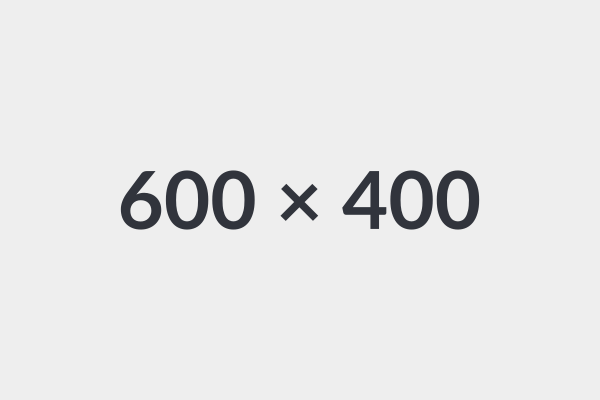
\includegraphics[height=2.5in]{images/placeholder.png}
	\caption{Synchronous Iteration and Synchronous Communication}
    \label{fig:SISC}
\end{figure}

This model appears to be well suited for parallel machines where all the computing units are of the same computing power, receive the same workload and the inter-communication between those computing units is a high speed connection. No idle time is expected in these conditions. Meanwhile, when  faced with an heterogeneous environment ( hardware and network heterogeneity),  this model can perform poorly. Notably, the first problem is the difference of computing power in the environment implying that with the same workload, computing units with more computing power will end their sub-task as quickly as they can while those with less power will take more time. This induce some idle time as some computing units despite having send their data to others, need to wait to receive the data corresponding to iteration k. Furthermore, computing units can be connected with different types of network showing different bandwidth, latency …. This add more idle time as data is not transmitted at the same speed.  To sum up, the SISC model is not expected to perform well on systems like local clusters or distributed systems that often rely on heterogeneous infrastructures and furthermore, not good for large problems. A workaround could be to minimize the idle time by overlapping computations and communication. 

\section{SIAC model}

[talk about convergence condition maybe with references]
The SIAC model rely on a subtle workaround despite being really close to the SISC and sequential scheme. In fact this model suggests the asynchronicity of communication, meaning that the computations and communication can be overlap. Given a set of data dependency, as soon as part of this data is computed on one computing unit, it's send to other computing units, then the computation should progress to complete the computation of all data dependencies. It's worth noting that the sending operation is not blocking, only the receiving operation is blocking in order to make sure that each process unit possess all data needed for the next iteration. [The effect of high latency network is diminished ]. Consequently, the idle time is minimize even though not suppress. As mentionned earlier, given the same distributed workload the most computational powered computing unit steal needs to wait for other non powerful computing units to compute all their data and send them before moving to the next iteration. Figure~\ref{fig:SIAC} illustrate this behavior.


\begin{figure}[htbp]
	\centering
	\captionsetup{justification=centering}
	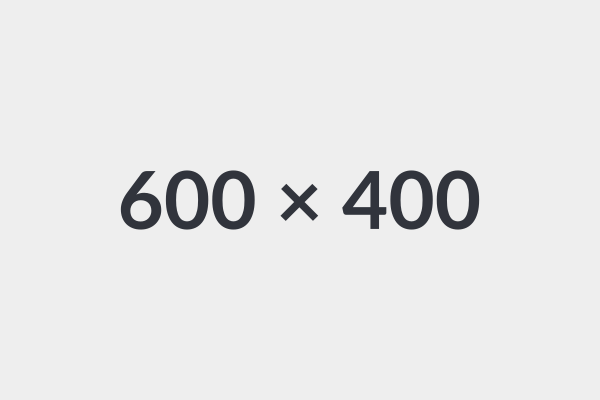
\includegraphics[height=2.5in]{images/placeholder.png}
	\caption{Synchronous Iteration and Aynchronous Communication}
    \label{fig:SIAC}
\end{figure}

To sum up, even though the idle time is minimize, it is not zeroed by this mechanism of asynchronous communication. The same assumptions hold for this scheme as far as distributed system is concerned: SIAC is need another level of asynchrony to fully harness the infrastructure.


\section{AIAC model}

[ajouter ici que le nombre d'iterations peut augmenter pour l'obtention de la convergence, mais que cette augmentation vaut mieux que le retard accusé par les systems synchrones, surtout dans des environnements ou le reseau est très congestionné ou defaillant]
The asynchronous iteration and asynchronous communication scheme also called the asynchronous iteration model is the global behavior of an algorithm that does not need any synchronization step whether at the iteration level of communication level, iterations and communication are all asynchronous. Rather than waiting for updates like in previous schemes, the computing unit just keep working with the last updates it receives, until new data arrive asynchronously to be consumed. In this context, the previously mentioned idle time is completely suppressed as shown by figure~\ref{fig:AIAC}


\begin{figure}[htbp]
	\centering
	\captionsetup{justification=centering}
	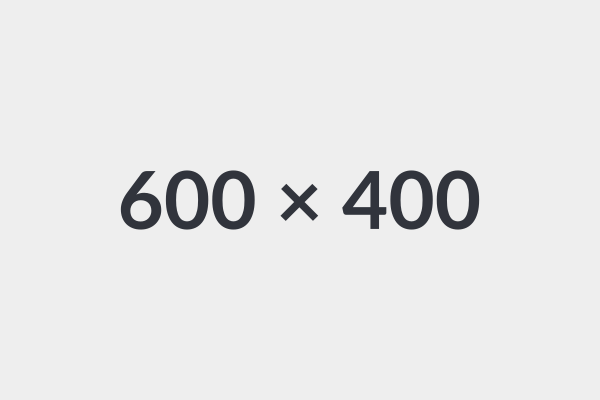
\includegraphics[height=2.5in]{images/placeholder.png}
	\caption{Aynchronous Iteration and Aynchronous Communication}
    \label{fig:AIAC}
\end{figure}

Assuming communications are now asynchronous and consequently free to be performed at any level of the algorithm, one can legitimately ask for performances purposes, when, where to send or receive data, and how to group data for efficient communication. Theses questions lead to a practical classification of AIAC algorithms in two classes: Semi-flexible communication AIAC and flexible communication AIAC models.

\subsubsection{Semi-flexible communication}


Semi-flexible communication refers to AIAC algorithms that has some restrictions over communication behavior, whether on the sender computing unit or on the receiver computing unit. This difference actually leads to two distincts sub-classes:


\begin{description}

    \item[Sender-side semi-flexibility] As the sub-class name suggests, the communication restrictions operate on the sender side. On the receiver side, no changes is to be noted. The receiver computing unit receives the updates during the iteration or at the end of the iteration, but only integrates the new data during the next iteration. On the sender side, the updates are sent as soon as the are available, preferably by group of data, to avoid network congestion. The ultimate goal of this scheme is to speed up the convergence process. Figure~\ref{fig:AIAC-sender-semi-flexible} illustrate this behavior.
    
    \item[Receiver-side semi-flexibility] Conversely to the previous sub-class, it’s the sender that does keep a rigid behavior and the receiver that has a flexible one. In fact the sender only send all the data necessary for updates at the end of every iteration. On the receiver side, the data reception is done as soon as the update is available, and the new data is integrated in the process of the computation on the same iteration if possible.Figure~\ref{fig:AIAC-receiver-semi-flexible} illustrate this behavior.
\end{description}


\begin{figure}[htbp]
	\centering
	\captionsetup{justification=centering}
	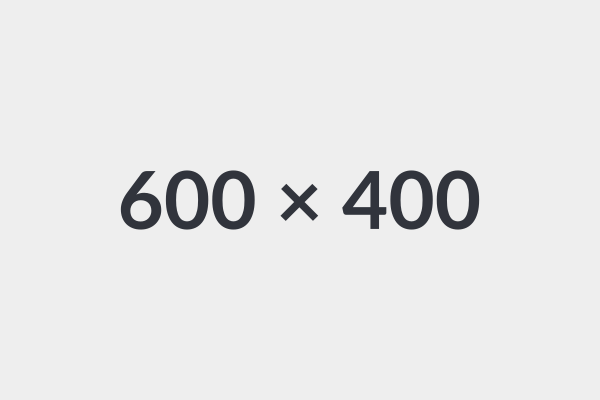
\includegraphics[height=2.5in]{images/placeholder.png}
	\caption{Sender-side semi-flexibility}
    \label{fig:AIAC-sender-semi-flexible}
\end{figure}


\begin{figure}[htbp]
	\centering
	\captionsetup{justification=centering}
	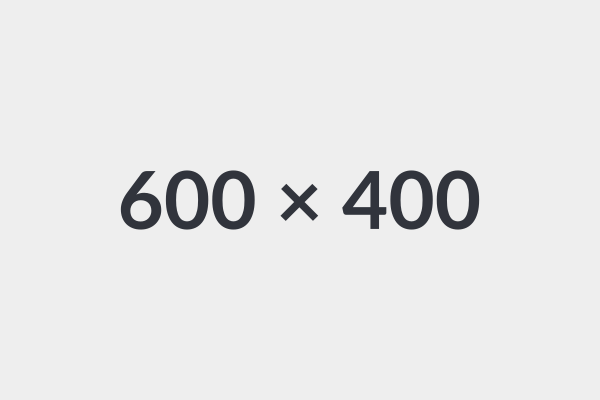
\includegraphics[height=2.5in]{images/placeholder.png}
	\caption{Receiver-side semi-flexibility}
    \label{fig:AIAC-receiver-semi-flexible}
\end{figure}


\subsubsection{Flexible communication}

The flexible communication scheme allow every computing unit to send data dependencies as soon as available on the sender side, and the on the receiver side, receive and integrate in the same iterations the new data available.Figure~\ref{fig:AIAC-flexible} illustrates this behavior.


\begin{figure}[htbp]
	\centering
	\captionsetup{justification=centering}
	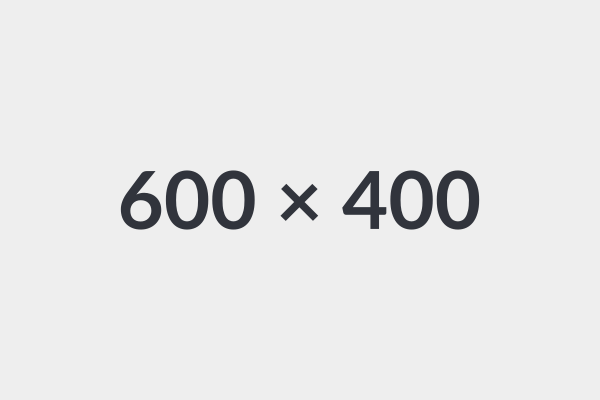
\includegraphics[height=2.5in]{images/placeholder.png}
	\caption{Receiver-side semi-flexibility}
    \label{fig:AIAC-flexible}
\end{figure}

\section{Convergence conditions and detection}


\todo{detection de convergence centralisé classique + detection de convergence distributé comme dans le livre}

\section{Programming environments}
\subsection{Dedicated programming environments}
\subsection{Non-dedicated programming environments}


\section{Conclusion}
% % \section{Stationary Iterative Methods for Solving Linear Systems}

% General Iteration Scheme and Matrix Splitting

% For a linear system $A\mathbf{x}=\mathbf{b}$ with $A \in \mathbb{R}^{n\times n}$, stationary iterative methods generate a sequence of approximations ${\mathbf{x}^{(k)}}$ to the solution by a fixed linear recurrence. The idea is to split the coefficient matrix $A$ into two parts, $A = M - N$, where $M$ is chosen to be easily invertible (e.g. diagonal or triangular) and $N = M - A$  . Using this splitting, the system $A\mathbf{x}=\mathbf{b}$ can be rewritten as $M\mathbf{x} = N\mathbf{x} + \mathbf{b}$, leading to the iterative update formula (assuming $M$ is nonsingular):

% \begin{equation}
% \mathbf{x}^{(k+1)} = M^{-1}\Big( N\,\mathbf{x}^{(k)} + \mathbf{b}\Big)\,. \tag{1}
% \end{equation}

% This is the general stationary iteration scheme  . We start from an initial guess $\mathbf{x}^{(0)}$ and apply (1) repeatedly. The method is called stationary because the iteration matrix $B = M^{-1}N$ and the vector $M^{-1}\mathbf{b}$ remain the same at each step (in contrast to more advanced nonstationary methods where the update changes with $k$). The error at step $k$ is $\boldsymbol{\epsilon}^{(k)} = \mathbf{x}^{(k)} - \mathbf{x}$ (with $\mathbf{x}$ the true solution). Subtracting the true solution from (1) gives $\boldsymbol{\epsilon}^{(k+1)} = M^{-1} N,\boldsymbol{\epsilon}^{(k)} = B,\boldsymbol{\epsilon}^{(k)}$. Thus the error evolves as $\boldsymbol{\epsilon}^{(k)} = B^k ,\boldsymbol{\epsilon}^{(0)}$. For convergence from any initial guess, we require $\boldsymbol{\epsilon}^{(k)} \to \mathbf{0}$ as $k\to\infty$, which is equivalent to $B^k \to 0$. Necessary and sufficient condition: the spectral radius of $B$ must be less than 1 :

% \begin{equation}
    
% \rho(B) < 1 \implies B^k \to 0 \text{ as } k\to\infty\,. \tag{2}
% \end{equation}

% In fact, $\rho(B)<1$ is the condition for convergence of the iteration for any $\mathbf{x}^{(0)}$ . In practice, it is often difficult to compute $\rho(B)$, so one uses sufficient conditions: if one can find a matrix norm $|\cdot|$ such that $|B| < 1$, then $|B^k| \le |B|^k \to 0$ as $k\to\infty$, guaranteeing convergence (by the Banach fixed-point theorem). Classic criteria like diagonal dominance ensure this. For example, if $A$ is strictly diagonally dominant by rows, one can show $|B|_\infty < 1$ for the iteration matrix $B$ of both Jacobi and Gauss–Seidel methods, hence convergence . We will discuss specific convergence conditions for each method later on.

% The efficiency of a stationary method depends on how $A$ is split. The matrix $M$ should be easy to invert (solving $M\mathbf{y}=\mathbf{c}$ should be much cheaper than solving $A\mathbf{y}=\mathbf{c}$ directly) . Common choices are:
% 	•	$M =$ diagonal part of $A$ (leads to the Jacobi method),
% 	•	$M =$ triangular part of $A$ (leads to Gauss–Seidel),
% 	•	or more generally $M =$ diagonal part scaled by a factor plus one triangular part (leads to Successive Over-Relaxation, SOR).

% These choices yield the classical stationary methods discussed below. Each method results in a specific iteration matrix $B = M^{-1}N$. The rate of convergence is determined by $\rho(B)$ (smaller is better), and the method converges if $\rho(B)<1$. We now derive the Jacobi, Gauss–Seidel and SOR methods via different matrix splittings and examine their properties.

% Jacobi Method

% The Jacobi method is the simplest stationary iterative solver for $A\mathbf{x}=\mathbf{b}$. It splits $A$ into its diagonal $D$ and off-diagonal parts $L$ and $U$ (strictly lower and strictly upper triangular, respectively):

% \begin{equation}
    
% A = D + L + U,
% \end{equation}

% where $D = \operatorname{diag}(a_{11},a_{22},\dots,a_{nn})$. In the Jacobi splitting, we take $M = D$ and $N = -(L+U)$, so that $M - N = D - (-(L+U)) = D + L + U = A$. Plugging into (1), we get the Jacobi iteration:

% \begin{equation}
    
% \mathbf{x}^{(k+1)} = D^{-1}\Big(\mathbf{b} - (L+U)\,\mathbf{x}^{(k)}\Big)\,. \tag{Jacobi}
% \end{equation}

% This means each component $x_i$ is updated using only values from the previous iteration:

% \begin{equation}
    
% x_i^{(k+1)} = \frac{1}{a_{ii}}\Big(b_i - \sum_{j\neq i} a_{ij}\,x_j^{(k)}\Big), \qquad i=1,2,\ldots,n .
% \end{equation}

% In other words, one Jacobi iteration computes the new $x_i^{(k+1)}$ by “solving” the $i$-th equation of $A\mathbf{x}=\mathbf{b}$ for $x_i$, assuming all other components $x_j$ (with $j\ne i$) are fixed to their old values from iteration $k$. The method can be implemented in a vectorized way using the formula above, or component-wise as given. Because each $x_i^{(k+1)}$ uses only the old iterate $\mathbf{x}^{(k)}$, Jacobi updates can be done in parallel for all $i$ – one does not overwrite $\mathbf{x}^{(k)}$ until the entire new vector $\mathbf{x}^{(k+1)}$ is computed . This requires storing two vectors (for old and new values), but allows straightforward parallelization across $n$ equations.

% Convergence and properties: The Jacobi iteration matrix is $B_J = D^{-1}(L+U) = I - D^{-1}A$. Its convergence requires $\rho(B_J)<1$ . A sufficient condition is that $A$ be strictly diagonally dominant (or irreducibly diagonally dominant) , i.e. $|a_{ii}| > \sum_{j\neq i}|a_{ij}|$ for each $i$. In that case $|B_J|_\infty < 1$ and Jacobi converges. In fact, diagonal dominance is often used as an easy check for convergence of both Jacobi and Gauss–Seidel  . Jacobi can sometimes converge even if these conditions are not met , but convergence is not guaranteed in general. Notably, Jacobi does not always converge for symmetric positive definite (SPD) matrices : SPD is not a sufficient condition by itself. For example, the SPD matrix

% \begin{equation}
    
% A=\begin{pmatrix}29 & 2 & 1\\ 2 & 6 & 1\\ 1 & 1 & \frac{1}{5}\end{pmatrix}
% \end{equation}

% has a Jacobi iteration matrix with $\rho(B_J)\approx 1.0661>1$, so the Jacobi method diverges in this case . (In technical terms, for Jacobi to converge on an SPD matrix $A$, $A$ must be diagonally dominant enough; one sufficient condition is that both $A$ and $2D - A$ are SPD .) In practice, Jacobi is usually slower to converge than Gauss–Seidel for the same matrix if both converge. However, Jacobi’s simplicity and parallelism can be advantages. It is sometimes used as a smoother in multigrid methods or as a preconditioner, despite its relatively slow convergence, because each iteration is cheap and easily parallelizable.

% Gauss–Seidel Method

% The Gauss–Seidel method improves upon Jacobi by using the most recently updated values as soon as they are available, instead of waiting for the next iteration. It corresponds to the splitting $A = (D+L) - U$, i.e. $M = D+L$ (the lower triangular part of $A$ including the diagonal) and $N = U$ (the strictly upper part). The iteration (1) then becomes:

% \begin{equation}
    
% (D+L)\,\mathbf{x}^{(k+1)} = \mathbf{b} - U\,\mathbf{x}^{(k)}\, ,
% \end{equation}

% so that we solve a triangular system each step:

% \begin{equation}
    
% \mathbf{x}^{(k+1)} = (D+L)^{-1}\Big(\mathbf{b} - U\,\mathbf{x}^{(k)}\Big)\,. \tag{Gauss–Seidel}
% \end{equation}

% This can be written component-wise as a forward sweep through $i=1$ to $n$:

% \begin{equation}
    
% x_i^{(k+1)} = \frac{1}{a_{ii}}\Big(b_i \;-\; \sum_{j< i} a_{ij}\,x_j^{(k+1)} \;-\; \sum_{j> i} a_{ij}\,x_j^{(k)}\Big), \qquad i=1,2,\ldots,n  .
% \end{equation}

% Here we use the newest available values: when computing $x_i^{(k+1)}$, all “previous” components $x_1^{(k+1)},\dots,x_{i-1}^{(k+1)}$ have already been updated in the current iteration, while $x_{i+1}^{(k)},\dots,x_n^{(k)}$ are still from the old iteration. In matrix form, $L\mathbf{x}^{(k+1)} = \mathbf{b} - U\mathbf{x}^{(k)}$ (with $L=D+L$ including the diagonal) . This asynchronous update tends to incorporate new information faster than Jacobi. Practically, Gauss–Seidel can be done in-place (overwriting) a single vector as we iterate $i=1$ to $n$, since once $x_i^{(k+1)}$ is computed, we will not need $x_i^{(k)}$ again.

% Convergence and properties: The Gauss–Seidel iteration matrix is $B_{GS} = (D+L)^{-1}U$. Gauss–Seidel often converges under similar conditions to Jacobi, and in fact it converges under somewhat weaker conditions. A sufficient condition for convergence is again strict or irreducible diagonal dominance of $A$ . More importantly, if $A$ is symmetric positive definite, Gauss–Seidel is guaranteed to converge  (in contrast to Jacobi). In general, whenever the Jacobi method converges, the Gauss–Seidel method will also converge and usually at a faster rate  . The reason is that $\rho(B_{GS})\le \rho(B_J)$ for the same matrix, often strictly smaller . Intuitively, by using fresher data, Gauss–Seidel reduces the error more per iteration. In fact, for many SPD matrices one can show $\rho(B_{GS}) = [\rho(B_J)]^2$ (see Convergence Analysis below), suggesting Gauss–Seidel squares the convergence factor of Jacobi, which is a significant improvement.

% On the downside, Gauss–Seidel’s updates are sequential and depend on the ordering of the unknowns. You cannot update all $i$ in parallel, which makes it less suitable for parallel computing compared to Jacobi . (There are techniques like coloring or domain decomposition to parallelize Gauss–Seidel by grouping independent updates, but the method is inherently sequential in a given ordering.) Another consideration is that different orderings of the equations or variables can affect the convergence speed of Gauss–Seidel. For certain matrices, a reverse order (sweeping $i=n$ down to $1$, sometimes called backward Gauss–Seidel) might perform similarly; doing one forward and one backward sweep gives the Symmetric Gauss–Seidel iteration, often used in analysis and as a preconditioner. In any case, the simplicity of Gauss–Seidel (just a triangular solve each iteration) and its typically better convergence per step than Jacobi make it a popular choice for many problems, especially if one can afford sequential updates.

% Successive Over-Relaxation (SOR)

% Successive Over-Relaxation (SOR) is a one-parameter generalization of Gauss–Seidel that can accelerate convergence by over-correcting the solution at each step. The method introduces a relaxation factor $\omega>0$. For $\omega=1$, SOR reduces to the Gauss–Seidel method; for $\omega \neq 1$, the update is a weighted combination of the old iterate and the would-be Gauss–Seidel update. Formally, the SOR iteration can be derived by splitting $A$ as:
% \begin{equation}
    
% A = \frac{1}{\omega}D + L \;-\; \Big(\frac{1-\omega}{\omega}D + U\Big).
% \end{equation}

% Here $M = \frac{1}{\omega}D + L$ (a lower triangular matrix) and $N = \frac{1-\omega}{\omega}D + U$. Plugging into the general iteration (1) yields:

% \begin{equation}
    
% (D + \omega L)\,\mathbf{x}^{(k+1)} \;=\; \omega\,\mathbf{b} - [\,\omega U + (\omega - 1)D\,]\,\mathbf{x}^{(k)} ,
% \end{equation}

% so that

% \begin{equation}
    
% \mathbf{x}^{(k+1)} \;=\; (D+\omega L)^{-1}\Big(\omega\,\mathbf{b} - [\,\omega U + (\omega - 1)D\,]\,\mathbf{x}^{(k)}\Big)\,. \tag{SOR}
% \end{equation}

% This can be understood as solving a modified triangular system at each step. It is instructive to look at the element-wise formula for SOR (with the forward sweep assumption as in Gauss–Seidel):


% \begin{equation}
% x_{i}^{(k+1)} \;=\; (1-\omega)\,x_{i}^{(k)} \;+\; \frac{\omega}{a_{ii}}\Big(b_{i} - \sum_{j<i}a_{ij}\,x_{j}^{(k+1)} - \sum_{j>i}a_{ij}\,x_{j}^{(k)}\Big), \qquad i=1,2,\ldots,n .
% \end{equation}
% The term in parentheses is precisely the Gauss–Seidel update for $x_i$ (the value it would have if we did a normal Gauss–Seidel iteration), and SOR takes a weighted average between the old value $x_i^{(k)}$ and this new Gauss–Seidel value. If $\omega=1$, we take the new value fully (recovering Gauss–Seidel). If $1 < \omega < 2$, we over-relax by taking the new value and then extrapolating a bit further in that direction – hopefully converging faster. If $0 < \omega < 1$, this is under-relaxation, meaning we move more cautiously toward the new value (this can be useful if $\omega=1$ was unstable or to slow down oscillations in the iteration). Note that $\omega$ outside the range $(0,2)$ is generally not useful: $\omega \ge 2$ usually causes divergence, and $\omega = 0$ is trivial (no update at all).

% In matrix terms, the SOR iteration matrix can be written as $B_{\omega} = (D+\omega L)^{-1}[(1-\omega)D - \omega U]$ (which reduces to $(D+L)^{-1}U$ for $\omega=1$, consistent with Gauss–Seidel) . The freedom to choose $\omega$ allows one to tune the spectral radius $\rho(B_{\omega})$. In fact, SOR includes Jacobi as an extreme case: if we let $\omega \to 1$ from below, we approach Gauss–Seidel; if we consider $\omega$ very large, the effect is to almost ignore $L$ (since $D+\omega L \approx \omega L$ for large $\omega$) and one can show the iteration approaches the Jacobi method in the limit $\omega\to\infty$ . Thus $\omega$ “interpolates” between different schemes, and for each problem there is an optimal $\omega$ (within $(0,2)$) that minimizes $\rho(B_{\omega})$.

% Convergence and properties: Just as with Gauss–Seidel, SOR converges under broad conditions. If $A$ is symmetric positive definite, SOR converges for any $0 < \omega < 2$  (this classic result was proved by Ostrowski in 1947). In fact, $\omega=1$ (Gauss–Seidel) and $\omega=2$ are the endpoints of convergence for SPD matrices – the spectral radius $\rho(B_{\omega})$ as a function of $\omega$ is < 1 for $\omega\in(0,2)$ and hits 1 at $\omega=2$ . For strictly diagonally dominant matrices, SOR is also convergent for a wide range around $\omega=1$ (typically $(0,2)$ as well) . However, the optimal choice of $\omega$ can greatly affect the speed of convergence (it “stretches” or contracts the spectrum of $B_{\omega}$). If $\omega$ is too low, we are under-relaxing and convergence is safe but slower than necessary; if $\omega$ is too high (close to 2), we over-relax too much and the method may become unstable or sluggish.

% The challenge is that the optimal $\omega$ depends on the spectral properties of $A$ (or of the related iteration matrices). In some special cases, one can estimate it. For instance, if we denote $\mu = \rho(B_J)$ the spectral radius of the Jacobi iteration for $A$, and assume the eigenvalues of $B_J$ are real, theory shows the optimal $\omega$ satisfies roughly $\omega_{\text{opt}} \approx \frac{2}{1+\sqrt{1-\mu^2}}$ . The corresponding minimal spectral radius is $\rho(B_{\omega_{\text{opt}}}) = \frac{1-\sqrt{1-\mu^2}}{1+\sqrt{1-\mu^2}}$, which for small $\mu$ is about $\mu^2/4$ . In particular, when $\omega=1$ (Gauss–Seidel), one can show $\rho(B_{GS}) = \mu^2$ under these assumptions . With $\omega_{\text{opt}}$, the spectral radius is roughly $(\mu^2)/4$, making SOR about four times more efficient than Gauss–Seidel in asymptotic error reduction . In less technical terms: SOR can dramatically speed up convergence if $\omega$ is well-chosen. In practice, one might try a few values of $\omega$ to see which gives the fastest decrease in residual or error. Values $\omega>1$ (over-relaxation) typically give faster convergence up to a point, while $\omega<1$ might be used if the method is diverging or wildly oscillatory (to damp changes). It’s worth noting that SOR, like Gauss–Seidel, is sequential and dependent on ordering. Also, for $\omega \neq 1$ the iteration matrix $B_{\omega}$ is not symmetric even if $A$ is symmetric, which means SOR is not directly usable as a preconditioner for the Conjugate Gradient method (which requires symmetric positive definite preconditioners). In such cases, one often uses a Symmetric SOR (SSOR) scheme – essentially a forward SOR sweep followed by a backward SOR sweep in each iteration – which yields a symmetric positive definite effective preconditioner. (SSOR as a standalone iterative method doesn’t improve convergence much over SOR , but it is very useful as a preconditioner for nonstationary methods like CG.)

% Convergence Analysis: Spectral Radius and Norm Criteria

% As derived earlier, the convergence of any stationary method $x^{(k+1)} = B x^{(k)} + \mathbf{c}$ hinges on the spectral radius $\rho(B)$. If $\rho(B)<1$, the iteration converges for any initial guess, and if $\rho(B)\ge 1$, in general it will diverge or at best stagnate . The error after $k$ steps is $\boldsymbol{\epsilon}^{(k)} = B^k \boldsymbol{\epsilon}^{(0)}$, so $|\boldsymbol{\epsilon}^{(k)}| \le |B^k|\cdot|\boldsymbol{\epsilon}^{(0)}|$. Submultiplicativity gives $|B^k| \le |B|^k$, so a sufficient condition for convergence is $|B|<1$. In practice, one uses an induced matrix norm that reflects some known matrix structure. For example, if $A$ is strictly diagonally dominant by rows, one can use the infinity-norm: each row $i$ of $B_J = D^{-1}(L+U)$ has sum of absolute values $\frac{1}{|a_{ii}|}\sum_{j\neq i}|a_{ij}| < 1$, thus $|B_J|\infty<1$ which guarantees $\rho(B_J)\le |B_J|\infty < 1$ and convergence . Similarly, diagonal dominance by columns would ensure $|B|_1<1$. These norm criteria are often how convergence conditions are proved.

% For Jacobi and Gauss–Seidel methods, diagonal dominance of $A$ is a convenient sufficient condition for convergence (and for Gauss–Seidel, even a bit weaker condition can suffice, e.g. $A$ being an $H$-matrix with positive diagonal entries). In addition, symmetric positive definiteness of $A$ guarantees convergence of Gauss–Seidel (and SOR) but not of Jacobi  . SPD matrices have a nice property for Gauss–Seidel: one can show that $\rho(B_{GS})<1$ by an energy argument (Gauss–Seidel can be seen as a damped gradient descent for an SPD system, making it convergent). In contrast, Jacobi on an SPD matrix may fail if the matrix is not sufficiently diagonally dominant (as we saw in the counterexample). In summary:
% 	•	Jacobi method: Converges if $A$ is strictly (or irreducibly) diagonally dominant . It may also converge under other conditions (e.g. $A$ and $2D-A$ both SPD ), but not for all SPD matrices. If Jacobi converges, it is usually the slowest of the three methods.
% 	•	Gauss–Seidel method: Converges if $A$ is strictly (or irreducibly) diagonally dominant (same condition as Jacobi) and in many cases when $A$ is symmetric positive definite . In fact, any SPD matrix yields convergence of GS . Gauss–Seidel often converges in cases where Jacobi does not. If Jacobi converges, Gauss–Seidel will too, and typically faster .
% 	•	SOR method ($\omega$ in (0,2)): Converges for any symmetric positive definite $A$ if $0<\omega<2$ . Also converges for $A$ strictly diagonally dominant (with an appropriate range of $\omega$ which usually includes $(0,2)$) . In general, SOR shares convergence conditions with Gauss–Seidel when $\omega$ is in the safe range. However, an $\omega$ significantly greater than 1 can destabilize the iteration if $A$ doesn’t meet those strong conditions, so one must choose $\omega$ carefully. When $A$ is SPD, we have the guarantee that any $0<\omega<2$ works , and we can then worry about optimizing $\omega$ for speed.

% Finally, a note on rate of convergence: if $\rho(B)=\rho < 1$, the asymptotic convergence is linear and the error after $k$ iterations behaves like $|\boldsymbol{\epsilon}^{(k)}| \approx \rho^k |\boldsymbol{\epsilon}^{(0)}|$ for large $k$. The quantity $-1/\ln \rho$ is essentially the number of iterations required to reduce the error by a constant factor. A smaller spectral radius $\rho$ means faster convergence. One can also consider the spectral radius as the definitive measure: for example, if method A has $\rho_A = 0.5$ and method B has $\rho_B = 0.25$, then asymptotically method B will reduce the error roughly twice as fast as method A (since $0.25^k = (0.5^k)^2$). In the next section, we compare Jacobi, Gauss–Seidel, and SOR in these terms and discuss practical implications.



% Spectral radius vs. relaxation factor in SOR: The spectral radius $\rho(C_\omega)$ of the SOR iteration matrix is plotted as a function of the relaxation factor $\omega$, for different values of the Jacobi-method spectral radius $\mu = \rho(C_{\text{Jac}})$ (blue, red, and green curves correspond to different $\mu$) . SOR achieves its fastest convergence at the optimal $\omega$ (where each curve attains minimum $\rho$). For smaller Jacobi spectral radius (blue curve), the optimal $\omega$ yields a very small $\rho(C_\omega)$, illustrating that SOR can greatly accelerate convergence (spectral radius near 0) compared to Gauss–Seidel ($\omega=1$ point) or Jacobi (whose $\rho=\mu$ is much larger). Conversely, if Jacobi is barely convergent ($\mu$ close to 1, green curve), the gain from SOR is modest and excessive $\omega$ can be detrimental (note the rise of the green curve as $\omega \to 2$).

% The Jacobi, Gauss–Seidel, and SOR methods each have their pros and cons. In terms of convergence speed per iteration, Gauss–Seidel is almost always superior to Jacobi when both converge. In many cases (especially for SPD matrices), one can roughly estimate $\rho_{GS} \approx (\rho_{Jacobi})^2$ . For example, if $\rho_{Jacobi}=0.9$, then $\rho_{GS}\approx 0.81$; if $\rho_{Jacobi}=0.5$, then $\rho_{GS}\approx 0.25$. This squared improvement means Gauss–Seidel can cut the number of iterations dramatically. Empirically, if Jacobi takes $K$ iterations to reach a certain error tolerance, Gauss–Seidel might take on the order of $K/2$ iterations (or even better), though this is a rough rule of thumb. The SOR method can further improve the rate: with an optimally chosen $\omega$, the spectral radius of SOR can be much smaller. In the theoretical scenario mentioned earlier, $\rho_{SOR} \approx \rho_{GS}/4$ at optimal $\omega$ , meaning SOR might take on the order of $K/4$ iterations compared to Gauss–Seidel’s $K/2$ (hence an order of magnitude fewer iterations than Jacobi in that scenario ). In practice, the actual speedup depends on $A$ and how close to optimal your $\omega$ is. Even without exact tuning, SOR with $\omega=1.1$ or $1.2$ often outperforms plain Gauss–Seidel significantly if the matrix is well-behaved.

% However, practical considerations beyond iteration counts also matter:
% 	•	Work per iteration: Jacobi and Gauss–Seidel both require on the order of $\mathcal{O}(n^2)$ operations per iteration for a dense $n\times n$ system (or $\mathcal{O}(nz)$ for a sparse matrix with $nz$ nonzeros). In Gauss–Seidel and SOR, the work is organized as a forward substitution (triangular solve). In Jacobi, it’s a matrix-vector multiply with $L+U$. The cost is similar, though Gauss–Seidel’s sequential nature can limit parallel efficiency. Jacobi’s simultaneous updates can take advantage of parallel hardware (all $n$ updates independent), whereas Gauss–Seidel and SOR have inherent data dependencies . On modern computing systems, this means Jacobi can often achieve better parallel speed-up, despite needing more iterations, whereas Gauss–Seidel might not scale well with many processors.
% 	•	Memory usage: Jacobi needs to store two vectors (old and new $x$) if implemented in the straightforward way, since it cannot overwrite $x^{(k)}$ as it computes $x^{(k+1)}$ . Gauss–Seidel (and SOR) can update in place, requiring only one vector of storage for $x$. For very large problems, this memory saving might be relevant (though one extra vector is usually negligible compared to storing $A$).
% 	•	Convergence reliability: Jacobi is the simplest but also the most fragile – it may fail to converge even when the other methods do. Gauss–Seidel is more robust (converges on SPD matrices, for instance, where Jacobi might not). SOR introduces a parameter: a poorly chosen $\omega$ can slow convergence or even cause divergence if $\omega$ is outside the allowable range. In practice, one might start with $\omega=1$ (Gauss–Seidel) and then try increasing $\omega$ to speed up convergence, but with caution not to approach the instability threshold (for SPD matrices this threshold is $\omega=2$). If $\omega$ is slightly suboptimal, SOR will still converge (if it converges at all) but not as fast as possible. Thus, there is a tuning aspect: methods like Jacobi and Gauss–Seidel are parameter-free, whereas SOR demands choosing $\omega$. The optimal $\omega$ might be estimated if one has some spectral information, or found by trial.
% 	•	Ordering and flexibility: Gauss–Seidel and SOR depend on the ordering of unknowns. This can be a disadvantage if the “natural” ordering of the problem is not ideal for convergence. For example, interchanging equations can change $\rho(B_{GS})$. There are strategies like reordering the matrix to be closer to diagonal dominance or to reduce bandwidth, which can improve convergence. Jacobi’s convergence factor is invariant to reordering of equations (since it treats all equations independently in parallel), so it’s conceptually simpler in that regard. In SOR, the optimal $\omega$ can even depend on ordering. For certain structured matrices (like those arising from 2D Poisson’s equation on a grid), the classic result is that SOR with lexicographic Gauss–Seidel order and an optimal $\omega$ achieves the best possible linear convergence for a local method, but one can also use red-black ordering (a two-color ordering) to allow parallel Gauss–Seidel updates which is equivalent to a form of Jacobi or SOR on a checkerboard pattern.
% 	•	Usage as preconditioners: While Jacobi, Gauss–Seidel, and SOR can be used as solvers on their own, today they are often used as preconditioners or smoothers in more advanced iterative methods (like Conjugate Gradient or multigrid). For example, Gauss–Seidel (especially in its symmetric variant) is a common smoother in multigrid algorithms, and SSOR is a popular preconditioner for Conjugate Gradient on SPD systems . Jacobi (diagonal scaling) is sometimes used as a simple preconditioner as well. In these roles, the relative convergence speeds and ordering issues still matter, but one also considers factors like how well they reduce certain components of error (smoothing properties) and their cost per iteration. Gauss–Seidel has good smoothing for high-frequency error components in PDE problems, whereas Jacobi is cheaper per step on parallel hardware.

% In summary, Gauss–Seidel is generally superior to Jacobi in convergence per iteration (often roughly twice as fast in practice)  , at the cost of being sequential. SOR can be much faster than Gauss–Seidel if an effective relaxation factor $\omega$ is chosen, sometimes yielding an order of magnitude speed-up . However, SOR requires tuning and shares Gauss–Seidel’s sequential nature and sensitivity to ordering. All three methods are linear convergence (no “acceleration” in the sense of CG’s finite termination on SPD matrices), and for very large or ill-conditioned systems, even SOR may converge slowly, prompting the use of more sophisticated algorithms. Nevertheless, understanding Jacobi, Gauss–Seidel, and SOR is fundamental, as they illustrate how using partial information (diagonal or triangular part of $A$) can lead to iterative solvers, and they form building blocks for modern techniques. Their convergence conditions (diagonal dominance, SPD, etc.) are commonly checked to ensure the iterations will converge. In practice, one would choose based on the problem: Jacobi if parallelization is crucial and the matrix is well-conditioned or diagonally dominant; Gauss–Seidel if a bit more speed is needed and one can handle sequential updates; SOR if further speed is desired and some trial-and-error with $\omega$ is acceptable. And if even more speed is required, one might move beyond stationary methods to conjugate gradients or multigrid, possibly using these classical methods as components (preconditioners or smoothers) within those frameworks .





% \section{Iterative Non-Stationary Methods for Solving Linear Systems}

% Introduction

% Solving a linear system $A\mathbf{x}=\mathbf{b}$ is a fundamental task in computational mathematics. For small systems or well-behaved matrices, direct methods (like Gaussian elimination or LU factorization) can find exact solutions in finite steps. However, for large-scale or sparse systems (with millions of unknowns), direct solvers become prohibitively expensive in memory and time  . In such cases, one turns to iterative methods, which generate a sequence of approximations $\mathbf{x}^{(k)}$ converging to the true solution $\mathbf{x}^*$. These methods update an initial guess $\mathbf{x}^{(0)}$ repeatedly to reduce the residual $\mathbf{r}^{(k)} = \mathbf{b} - A\mathbf{x}^{(k)}$. Iterative algorithms are often the only feasible option for extremely large or complex systems arising from applications like discretized PDEs, optimization, or machine learning .

% Stationary vs. Non-Stationary Iterations: Iterative techniques fall into two broad categories: stationary methods and non-stationary methods  . In a stationary iterative method, the update formula is fixed and does not change with $k$. One can write the iteration as:
% \begin{equation}
    
% \mathbf{x}^{(k+1)} = B\,\mathbf{x}^{(k)} + \mathbf{c},
% \end{equation}

% where $B$ and $\mathbf{c}$ are fixed matrix and vector, independent of the iteration count . Examples include the Jacobi and Gauss–Seidel relaxations, where $B = M^{-1}N$ for some fixed splitting $A=M-N$ . These methods are simple and memory-efficient, but they often converge slowly and only under certain conditions (e.g. diagonal dominance or positive-definiteness of $A$)  . By contrast, non-stationary (or Krylov subspace) methods use information that changes at each iteration, such as the current residual, to adapt their next step . Their update formulas involve iteration-dependent coefficients (often obtained via inner products of residuals or search directions), making the process non-linear in the error. These methods are usually more sophisticated and effective, converging in far fewer steps than stationary schemes for difficult problems . For example, the conjugate gradient (CG) method – a non-stationary Krylov method for symmetric positive-definite matrices – can find the solution in a nearly optimal path, in stark contrast to simpler stationary approaches (like fixed-step steepest descent). This is illustrated in Figure 1, where the red path (CG) reaches the solution $\mathbf{x}$ in a direct zig-zag route, whereas the green path (gradient descent) makes slow orthogonal progress



% . In general, non-stationary methods harness more algebraic structure of $A$ at each step (such as previous search directions or residuals) to accelerate convergence, at the cost of a more complex analysis and implementation .

% Theoretical Foundation: Stationary vs. Non-Stationary Methods

% Stationary Iterative Methods. A linear stationary iteration for $A\mathbf{x}=\mathbf{b}$ can be derived by splitting $A = M - N$, with $M$ chosen for easy inversion . The iteration is then $M,\mathbf{x}^{(k+1)} = N,\mathbf{x}^{(k)} + \mathbf{b}$, or $\mathbf{x}^{(k+1)} = \mathbf{x}^{(k)} + M^{-1}(\mathbf{b} - A\mathbf{x}^{(k)})$ . Here, $M^{-1}N = I - M^{-1}A$ plays the role of a constant iteration matrix $C$ so that $\mathbf{e}^{(k+1)} = C,\mathbf{e}^{(k)}$ (where $\mathbf{e}^{(k)}=\mathbf{x}^{(k)}-\mathbf{x}^*$ is the error)  . Convergence is guaranteed if and only if all eigenvalues of $C$ lie strictly inside the unit circle, $\rho(C)<1$ . This spectral radius condition typically holds for matrices $A$ that are diagonally dominant, symmetric positive definite, or satisfy related criteria, after an appropriate splitting. Classic stationary methods include Jacobi’s method, Gauss–Seidel, and Successive Over-Relaxation (SOR)  . These rely on algebraic properties like matrix splittings and usually converge linearly (if at all), often requiring preconditioning or acceleration to be practical for large systems. Notably, stationary schemes have fixed update coefficients (e.g. a fixed relaxation factor $\omega$ in SOR), and do not “learn” from past iterations beyond the last iterate. This simplicity makes them easy to analyze and implement, but also limits their speed of convergence  .

% Non-Stationary Iterative Methods. Non-stationary methods abandon the fixed iteration matrix paradigm and instead adapt at each step. In these methods, the sequence of corrections is constructed based on dynamically computed coefficients, often involving inner products of current and previous residuals or search directions . Equivalently, one can view many non-stationary solvers as applying a varying higher-degree polynomial in $A$ to the initial residual at each iteration (instead of repeatedly applying a fixed $B$). The coefficients of this polynomial are chosen on the fly to optimize some criterion (such as residual norm). This adaptive approach allows non-stationary methods to accelerate convergence dramatically by canceling out error components associated with troublesome eigenvalues of $A$. Indeed, non-stationary Krylov methods can converge in at most $n$ steps in exact arithmetic by constructing a polynomial that annihilates the error (since the Krylov space eventually spans the whole $\mathbb{R}^n$)  . In practice, rounding errors and very large $n$ mean convergence in $\ll n$ steps is desired; the success of these methods hinges on the spectral properties of $A$. Intuitively, if $A$’s eigenvalues (or singular values) are clustered or well-conditioned, Krylov methods find a good approximation quickly by resolving large-scale components of the error first . Conversely, if $A$ has a wide spread of eigenvalues or pathological structure, convergence may stall or slow down (this is where preconditioning becomes crucial – discussed later).

% Algebraically, most non-stationary methods can be understood as projection methods onto a sequence of subspaces that grow with each iteration. Unlike stationary iterations that rely on the spectral radius of a fixed matrix $C$, Krylov methods leverage properties like orthogonality, optimality, and conjugacy in these subspaces. This makes their convergence analysis more involved (depending on polynomial approximations to $A^{-1}$ and the entire spectrum of $A$ ), but also more powerful. In summary, stationary methods are often used as preconditioners or smoothers (e.g. Gauss–Seidel in multigrid) rather than standalone solvers, whereas the heavy lifting for difficult linear systems is done by non-stationary Krylov solvers which adaptively exploit $A$’s algebraic structure.

% Krylov Subspace Methods: Orthogonality, Residual Minimization, and Projections

% Most non-stationary iterative methods of interest are Krylov subspace methods. The Krylov subspace of dimension $k$ generated by matrix $A$ and initial residual $\mathbf{r}^{(0)} = \mathbf{b}-A\mathbf{x}^{(0)}$ is defined as:

% \begin{equation}
    
% \mathcal{K}_k(A,\mathbf{r}^{(0)}) = \mathrm{span}\{\mathbf{r}^{(0)},\,A\mathbf{r}^{(0)},\,A^2\mathbf{r}^{(0)},\dots,A^{k-1}\mathbf{r}^{(0)}\}\,.
% \end{equation}

% This is the space of all linear combinations of the first $k$ powers of $A$ applied to the initial residual . Krylov methods iterate by expanding this subspace and seeking an improved solution $\mathbf{x}^{(k)}$ in the affine space $\mathbf{x}^{(0)} + \mathcal{K}_k(A,\mathbf{r}^{(0)})$. At each step, they enforce a condition that defines the new approximation, typically a projection condition: the residual at step $k$, $\mathbf{r}^{(k)} = \mathbf{b}-A\mathbf{x}^{(k)}$, is made orthogonal to some subspace (the test subspace). By construction $\mathbf{x}^{(k)}$ lies in the trial subspace $\mathbf{x}^{(0)} + \mathcal{K}_k$, so the method is choosing the “best” vector in that Krylov space according to some optimality criterion.

% Two common choices of projection lead to different families of methods: (1) Galerkin (Petrov-Galerkin) orthogonality: enforce $\mathbf{r}^{(k)}$ orthogonal to the trial subspace itself (or to a closely related subspace), and (2) Residual minimization: choose $\mathbf{x}^{(k)}$ that explicitly minimizes $|\mathbf{r}^{(k)}|$ over all candidates in $\mathbf{x}^{(0)} + \mathcal{K}_k$. The conjugate gradient (CG) method is an example of the first approach (Galerkin): for SPD matrices, CG chooses $\mathbf{x}^{(k)}$ such that the residual is orthogonal to $\mathcal{K}_k$ (which, in CG, also equals orthogonality to all previous residuals) . Equivalently, CG ensures the error $\mathbf{e}^{(k)}=\mathbf{x}^{(k)}-\mathbf{x}^*$ is minimized in the $A$-norm (an energy norm) within the trial subspace. On the other hand, GMRES (Generalized Minimal Residual) is the prototypical residual-minimization method: it selects $\mathbf{x}^{(k)}$ that minimizes $|\mathbf{r}^{(k)}|_2$ over $\mathbf{x}^{(0)}+ \mathcal{K}_k$ . This is achieved by building an orthonormal basis of $\mathcal{K}_k$ (using the Arnoldi process) and solving a small least-squares problem each iteration to obtain the coefficients that minimize the residual norm  . Other Krylov methods use variations or combinations of these two approaches – for example, BiCG uses a Petrov-Galerkin condition with two different subspaces, and BiCGStab adds a local residual-minimizing step to the BiCG process.

% Orthogonality and Conjugacy: Krylov solvers heavily exploit orthogonal or conjugate directions to improve efficiency. In CG, the successive residuals $\mathbf{r}^{(k)}$ are made orthogonal to each other (in the Euclidean inner product) and the search directions $\mathbf{p}^{(k)}$ are constructed to be $A$-conjugate (mutually orthogonal with respect to the $A$-inner product)  . This conjugacy condition ensures that each iteration corrects errors along a new eigen-direction of $A$ without spoiling the progress on previous directions. Thanks to these properties, CG implicitly builds an orthonormal basis of the Krylov subspace with short recurrences – only the last two residuals and search directions are needed to generate the next direction. In contrast, for a general non-symmetric $A$, one cannot maintain orthonormality with such short recurrences . GMRES addresses this by the Arnoldi process: it explicitly orthogonalizes the new Krylov vector $A\mathbf{v}^{(k)}$ against all previous basis vectors ${\mathbf{v}^{(1)},\dots,\mathbf{v}^{(k)}}$ to maintain an orthonormal basis of $\mathcal{K}_k$  . The benefit is a guarantee that the residual $\mathbf{r}^{(k)}$ is perpendicular to $\mathcal{K}_k$ (hence $ |\mathbf{r}^{(k)}|_2$ is minimized) . The cost, however, is that GMRES requires long recurrences: storing all $k$ basis vectors and performing $O(k)$ work to orthogonalize each new vector, which becomes expensive as $k$ grows  .

% Other Krylov methods find compromises. BiCG (Bi-Conjugate Gradient) generates two coupled sequences of basis vectors: one for the Krylov subspace of $A$ (using the residual $\mathbf{r}^{(k)}$) and one for the Krylov subspace of $A^T$ (using a shadow residual $\tilde{\mathbf{r}}^{(k)}$) . It enforces a bi-orthogonality: the residuals from the $A$-sequence are orthogonal to the $A^T$-Krylov basis (which can be seen as a Galerkin condition with a different test subspace). This yields a short-recurrence method for non-symmetric $A$—like CG, only a few vectors are kept—but at the expense of potential breakdown (if the process encounters a situation where an inner product vanishes unexpectedly) . Variants like QMR (Quasi-Minimal Residual) apply additional techniques (least-squares smoothing of BiCG’s updates) to avoid breakdowns and smooth the convergence  . CGS (Conjugate Gradient Squared), described below, takes a different approach: it essentially squares the BiCG polynomial, eliminating the need for the $A^T$ sequence by merging it with the $A$-sequence . And BiCGStab (BiCG Stabilized) further refines BiCG/CGS by adding a one-step residual minimization (a small GMRES step of length 1) at each iteration to stabilize convergence  .

% Residual Minimization and Optimality: A hallmark of Krylov methods is that many of them are optimal in some sense. GMRES is $l_2$-optimal: at iteration $k$ it produces the smallest possible $|\mathbf{r}^{(k)}|_2$ among all linear combinations of ${I, A, \dots, A^{k-1}}$ applied to $\mathbf{r}^{(0)}$ . In other words, GMRES finds the best approximation in the $k$-dimensional Krylov space by a least-squares criteria. MINRES is similar for symmetric systems (minimizing residual in the $A$-norm for indefinite symmetric $A$). Conjugate Gradient is optimal in the $A$-norm (it minimizes the error norm $|\mathbf{e}^{(k)}|_A$ over the Krylov space for SPD $A$). This optimality leads to predictable convergence bounds: for CG one can prove

% \begin{equation}
    
% \|\mathbf{e}^{(k)}\|_A \;\le\; 2\left(\frac{\sqrt{\kappa(A)}-1}{\sqrt{\kappa(A)}+1}\right)^k \,\|\mathbf{e}^{(0)}\|_A,
% \end{equation}

% where $\kappa(A)$ is the condition number of $A$ . This shows the error drops at least as fast as $(\sqrt{\kappa}-1)/(\sqrt{\kappa}+1)$ per iteration (CG often converges faster than this worst-case bound due to spectral clustering or superlinear convergence when eigenvalues cluster ). GMRES lacks such a simple bound in terms of $\kappa(A)$, because for non-normal matrices the convergence can depend on the entire spectrum distribution and eigenvector conditioning. Nonetheless, GMRES will converge in at most $n$ steps (exact in $\mathbb{R}^n$) , and in practice often much sooner if the polynomial of best approximation of $A^{-1}$ on the spectrum is of low degree. Non-stationary methods are typically superior to stationary ones because they build these optimal (or near-optimal) polynomials adaptively, whereas a stationary method effectively applies the same fixed polynomial (the iteration matrix $C$) repeatedly, without targeting the troublesome spectral components of the error.

% Key Examples of Non-Stationary Iterative Methods

% Conjugate Gradient (CG) – prototype for SPD systems

% CG is the oldest and one of the most powerful non-stationary methods, applicable to symmetric positive-definite (SPD) matrices. It generates a sequence of conjugate (A-orthogonal) directions $\mathbf{p}^{(k)}$ and ensures the residuals $\mathbf{r}^{(k)}$ are orthogonal to each other . Each iteration chooses step lengths $\alpha_k$ and $\beta_k$ (via inner products of residuals) to minimize the quadratic error (since solving $A\mathbf{x}=\mathbf{b}$ for SPD $A$ is equivalent to minimizing a convex quadratic function). As a result, CG converges in at most $n$ steps, and in practice often in far fewer: the error after $k$ steps satisfies the bound above, which depends on $\sqrt{\kappa(A)}$ . If $A$’s eigenvalues cluster, convergence is significantly accelerated (sometimes superlinear). CG’s algorithmic structure is simple: each iteration does one matrix-vector multiply $A\mathbf{p}^{(k)}$, two inner products (to compute $\alpha_k$ and update $\beta_{k}$), and a few vector saxpy operations. Storage is minimal – it needs only a handful of $n$-vectors (for $\mathbf{x}^{(k)}$, $\mathbf{r}^{(k)}$, $\mathbf{p}^{(k)}$, and $A\mathbf{p}^{(k)}$), making it very memory-efficient. This combination of speed and low memory makes CG extremely effective for large SPD problems . Indeed, CG is often the method of choice for symmetric linear systems arising from e.g. finite element discretizations of elliptic PDEs (structural mechanics, diffusion problems, etc.), especially when a good preconditioner is available. The theoretical elegance of CG (polynomial optimality and three-term recurrence) set the stage for all later Krylov methods.

% Generalized Minimal Residual (GMRES) – robust solver for unsymmetric systems

% GMRES (Saad and Schultz, 1986) is a widely used method for general non-symmetric (or non-Hermitian) matrices. GMRES constructs an orthonormal basis ${v_1,\dots,v_m}$ for $\mathcal{K}_m(A,r^{(0)})$ via the Arnoldi process , and computes the new approximation $\mathbf{x}^{(m)} = \mathbf{x}^{(0)} + \sum_{j=1}^m y_j,v_j$ that minimizes $|\mathbf{b}-A\mathbf{x}^{(m)}|_2$. This leads to solving a small $m\times m$ least-squares problem (often written as $H \mathbf{y} \approx \beta e_1$ for the upper Hessenberg matrix $H$ obtained from Arnoldi)  . By design, GMRES produces the smallest residual norm possible after $m$ steps (among all Krylov methods of that subspace dimension) . This often gives it excellent robustness – GMRES will converge whenever the underlying Krylov subspace contains a good approximation, and it is guaranteed not to stagnate before reaching the true solution (except in pathological cases where the best polynomial approximation of $A^{-1}$ is the trivial one of degree $n$). In exact arithmetic GMRES would solve the system in $\le n$ steps ; in practice one uses restarted GMRES, denoted GMRES($m$), which limits the basis size to $m$ to control storage and orthogonalization cost  . For example, GMRES(30) restarts every 30 iterations (discarding the accumulated basis and starting anew from the current residual). Restarts prevent runaway memory use, but if chosen too small can hurt convergence or cause stagnation (failure to improve until $m$ is large enough)  . GMRES without restart has $O(nm + m^2)$ work per $m$ iterations (due to orthogonalization) and $O(nm)$ storage, which is why $m$ is kept moderate in practice.

% Advantages: GMRES is a “black-box” solver – it works on any square matrix (even singular ones in certain cases, with appropriate handling) and is often very stable. It excels for tough nonsymmetric problems where other methods (BiCG or CGS) might break down or exhibit wild residual oscillations. Disadvantages: The memory and CPU cost of the growing Arnoldi process. For very large $n$, GMRES($m$) with small $m$ might converge slowly, whereas large $m$ is infeasible. Strategies like adaptive restarting or augmenting the subspace with known troublesome vectors (e.g. eigenvector approximations) are used to mitigate this. Despite these issues, GMRES remains a workhorse in industrial solvers for problems like computational fluid dynamics (Navier–Stokes equations), where matrices are large, sparse, and non-symmetric, and a direct solve is impossible.

% Bi-Conjugate Gradient (BiCG) – extending CG to non-symmetric systems

% BiCG is a Krylov method that generalizes the conjugate gradient concept to matrices $A$ that are not symmetric. Since CG’s simplicity relies on the symmetry of $A$ (which guarantees a single Krylov sequence suffices), BiCG tackles the general case by generating two sequences of vectors: ${p_k}$ in the column space of $A$ and ${\tilde{p}_k}$ in the column space of $A^T$. It simultaneously advances these sequences such that they remain bi-orthogonal (i.e. $\tilde{p}_i^T (A,p_j) = 0$ for $i\neq j$), ensuring a Petrov-Galerkin condition: the residual $r^{(k)}$ is made orthogonal to the space spanned by ${\tilde{p}_1,\dots,\tilde{p}_k}$ . In practice, one can implement BiCG with a short two-term recurrence similar to CG, but requiring two matrix-vector multiplications per iteration: one with $A$ and one with $A^T$ . The need to multiply by $A^T$ is a drawback if $A$ is not readily transposable (e.g. when $A$ is given as a black-box operator or in a distributed format). BiCG’s cost per iteration is roughly twice that of CG (two matvecs, and a few dot-products) and it uses a small, fixed number of vectors for storage (on the order of 4–6 vectors of length $n$). Like CG, BiCG does not explicitly minimize any residual norm; thus its convergence can be irregular – residuals might fluctuate in norm. When it converges, BiCG often achieves a solution of accuracy comparable to GMRES in fewer iterations (but with each iteration costing more) . However, BiCG can suffer breakdown if at some step the direction vectors lose bi-orthogonality (denominator in recurrence becomes zero). Look-ahead strategies exist to overcome breakdowns at additional cost , but other methods were developed to improve upon BiCG’s reliability.

% Despite its pitfalls, BiCG is historically important and forms the backbone for more refined solvers. For instance, on SPD matrices BiCG reduces to CG (and indeed delivers identical results as CG, but at twice the work, making it inefficient for SPD cases) . BiCG is seldom used on its own today; instead one of its variants is preferred, as discussed next.

% Conjugate Gradient Squared (CGS) – squaring the BiCG polynomial for speed

% CGS (Sonneveld, 1989) was introduced to avoid the explicit computation with $A^T$ in BiCG and potentially double the convergence speed. The idea is clever: in BiCG, one can view the residual after $k$ steps as $r^{(k)} = P_k(A),r^{(0)}$ for some $k$-degree polynomial $P_k$. CGS considers $P_k^2(A),r^{(0)} = P_k(A),P_k(A),r^{(0)}$, effectively using the same polynomial for both $A$ and (implicitly) $A^T$ sequences . By interleaving the BiCG recurrences, CGS produces a new residual sequence that (in exact arithmetic) corresponds to the squared minimal polynomial of BiCG, ideally achieving the solution in roughly half as many iterations. In practice, CGS often does converge in fewer iterations than BiCG (roughly, it may finish in $k/2$ iterations compared to BiCG’s $k$) . Importantly, CGS does not require $A^T$ – it uses only $A$-multiplications, performing two of them per iteration (so the flops per iteration are similar to BiCG’s two matvecs, but without needing the transpose)  . This made CGS attractive for problems where forming $A^T$ is inconvenient.

% The major drawback of CGS is that squaring the polynomial can lead to highly irregular convergence . The residual norm in CGS sometimes oscillates wildly, even increasing temporarily or failing to decrease monotonically. This can cause loss of accuracy or instability in finite precision. In some cases, CGS can stagnate or diverge where BiCG would have converged steadily. Nonetheless, CGS was an important development because it eliminated the $A^T$ requirement and spurred research into fixes for the erratic convergence. Today, CGS is generally supplanted by BiCGStab (or variants like BiCGStab(l)), which we discuss next, but its idea of polynomial squaring is conceptually valuable.

% Bi-Conjugate Gradient Stabilized (BiCGStab) – smoothing and improving BiCG/CGS

% BiCGStab (van der Vorst, 1992) is one of the most popular general-purpose solvers for unsymmetric systems. It was designed specifically to cure the weaknesses of CGS while retaining its strengths  . BiCGStab starts from the BiCG two-sequence framework (like CGS does) but introduces an additional “stabilization” step in each iteration. In each BiCGStab iteration, one first performs a BiCG-like update (one $A$ matvec, producing an intermediate residual as in BiCG), and then follows up with a single-step GMRES minimization (one more $A$ matvec) restricted to the space spanned by the current residual and the $A$-applied residual . In effect, BiCGStab applies a degree-1 polynomial smoothing $Q_i(A)$ to the result of the BiCG iteration $P_i(A)$ . The smoothing polynomial $Q_i$ is chosen (via an inner product) to minimize the residual norm in that 2-dimensional subspace (often denoted by an $\omega_i$ parameter in the algorithm). The outcome is that residuals are much smoother – BiCGStab tends to avoid the extreme oscillations of CGS . In many cases BiCGStab’s convergence is also more reliable than BiCG, since it combines the fast convergence modes of BiCG with occasional damping.

% Each iteration of BiCGStab costs two $A$–multiplications (like CGS and BiCG) and a handful of dot-products and axpy operations. It also does not require $A^T$ (like CGS, it only uses $A$ on-the-fly). The storage overhead is small (a few vectors, similar to BiCG). Thus, per iteration cost and memory of BiCGStab are comparable to BiCG/CGS . The benefit is that BiCGStab often converges as fast or faster than CGS in practice and with far fewer erratic spikes in residual norm  . It is regarded as one of the best general-purpose Krylov solvers for nonsymmetric matrices when one wants a good balance of convergence speed, robustness, and low memory. There are further improvements like BiCGStab($\ell$) which apply an $\ell$-degree GMRES smoothing polynomial instead of 1 (giving more robust but sometimes slower convergence), and IDR(s) (Induced Dimension Reduction) methods that have fixed subspace recycling, but BiCGStab remains highly competitive for many problems.

% Summary of Algorithmic Structure: The table below summarizes and compares some features of these key methods:
% 	•	CG: short recurrences (2-term), one $A$ matvec per iteration; optimal for SPD matrices; storage ~4 vectors; convergence rate tied to $\sqrt{\kappa(A)}$.
% 	•	GMRES: long recurrences (full orthogonalization), one $A$ matvec per iteration; optimal residual in 2-norm; storage grows with iterations (or with restart length $m$); robust for general $A$ but cost grows and may need restarting.
% 	•	BiCG: short recurrences (2-term) but two coupled sequences; two matvecs ($A$ and $A^T$) per iteration; not norm-minimizing, residual can oscillate; storage ~6 vectors; works for general $A$ but can break down.
% 	•	CGS: short recurrences, no $A^T$ needed; two $A$ matvecs per iteration (like BiCG); often faster convergence in iterations than BiCG but with highly irregular residual behavior; storage ~6 vectors; rarely used now due to instability.
% 	•	BiCGStab: short recurrences, no $A^T$; effectively two $A$ matvecs per iteration; smoother convergence than CGS (and often BiCG); storage ~6–8 vectors; one of the most reliable choices for general unsymmetric systems.

% All these methods (except GMRES without restart) have $O(n)$ storage and $O(n)$ work per iteration plus the cost of matvecs (which is $O(\text{nnz}(A))$ for sparse $A$, or more if $A$ is dense). In modern high-performance computing, the matrix-vector multiply is usually the dominant cost, so methods with more matvecs per iteration (BiCG, CGS, BiCGStab) are a bit more expensive per step than ones with one matvec (CG, GMRES). However, they may converge in fewer iterations. There is also a consideration of communication overhead: methods like CG and BiCGStab require a couple of global inner products per iteration, which can limit scalability on parallel machines. Research into s-step Krylov methods and avoiding global synchronization is ongoing, but beyond our scope here.

% Convergence Properties and the Role of Preconditioners

% The convergence of non-stationary iterative methods is intricately linked to the spectrum of $A$ (its eigenvalues, and for non-normal $A$, the behavior of the pseudoeigenvalues as well). Roughly speaking, Krylov methods struggle when $A$ is ill-conditioned or has eigenvalues spread over a large range or lying on problematic locations in the complex plane. For example, CG’s error bound involves $\kappa(A) = \lambda_{\max}/\lambda_{\min}$; if this condition number is large, convergence is slow . GMRES’s performance can degrade if $A$ has eigenvalues on or near the unit circle or if $A$ is nearly defective (non-diagonalizable), causing the Krylov basis vectors to become almost linearly dependent. One often observes stagnation or extremely slow improvement in those cases. Convergence analysis is generally hard – for CG there is a rich theory involving Chebyshev polynomials and A-norm energy minimization, for GMRES and BiCG there are results relating residual polynomials to Faber or Leja points in the complex plane , but precise convergence rates are usually problem-specific.

% A few general statements can be made:
% 	•	Krylov methods will converge in $n$ steps in exact arithmetic (since $\deg p(A) \le n$ for the minimal polynomial)  , but round-off error effectively limits the useful subspace dimension and can cause stagnation before $n$ steps. Typically, one desires convergence in $k \ll n$ steps.
% 	•	Eigenvalue distribution: If the eigenvalues of $A$ cluster in a few intervals, a low-degree polynomial can approximate $1/A$ well on that spectrum, leading to fast convergence. Conversely, if eigenvalues are widespread, the residual polynomial needs higher degree. For CG, tightly clustered eigenvalues (except a few outliers) lead to superlinear convergence as the method “zeros out” whole clusters quickly. For GMRES/BiCG, a helpful metric is the field of values (numerical range) – if that is narrow or well-separated from the origin, convergence is faster. Indefinite or sign-changing spectra (for which some eigenvalues are very small or zero) pose challenges – CG will stagnate if any $\lambda_i=0$ (singular $A$) or if $\kappa$ is huge, etc.
% 	•	Non-normal matrices: Even if the eigenvalues suggest easy convergence, a highly non-normal matrix can cause slow convergence (GMRES in particular) because eigenvectors are not orthogonal and the Krylov basis may need to be large to capture the difficult directions. In such cases, residual norms don’t tell the full story of error (someone might see “delay” in convergence until certain invariant subspaces are approximated).

% To address slow convergence, one almost always employs a preconditioner $M$. A preconditioner is an auxiliary matrix (or operator) that approximates $A^{-1}$ in some sense, used to transform the linear system into one that is more favorable spectrally . Commonly $M$ is chosen such that $M^{-1}A$ (or $AM^{-1}$) has a smaller condition number or more clustered eigenvalues than $A$. Krylov methods can then be applied to the preconditioned system (e.g. solve $M^{-1}A x = M^{-1}b$ by iterations). Good preconditioners drastically improve convergence – for instance, a well-tuned Incomplete LU (ILU) or multigrid preconditioner can reduce the needed iterations by an order of magnitude or more. In effect, preconditioning incorporates some of the benefits of stationary methods (which split $A$ = preconditioner + remainder) into Krylov solvers . Indeed, one can view many Krylov methods as accelerated stationary iterations: e.g. preconditioned CG is like a polynomially accelerated form of the Jacobi or Gauss–Seidel method used as $M^{-1}$ . Preconditioning is a vast topic on its own – key points are that the preconditioner must be computationally cheap to apply (ideally one solve of $M$ per iteration, costing much less than solving $A$ directly) and should make $M^{-1}A$ spectrally friendly (clustered eigenvalues, low $\kappa(M^{-1}A)$, or deflated problematic modes).

% Convergence in practice: With a decent preconditioner, CG typically converges in $\mathcal{O}(\sqrt{\kappa(M^{-1}A)})$ iterations, often a small multiple of the problem’s dimension in the context of PDEs (e.g. for elliptic PDEs, multigrid can make iterations independent of $n$). GMRES and BiCGStab with preconditioning often show convergence profiles where the residual norm drops steadily (sometimes with a few stagnation plateaus that eventually resolve). One must be cautious: methods like BiCG and BiCGStab can still break down (e.g. if $M^{-1}A$ has certain eigenvalue distributions causing the BiCG formulas to hit a zero divisor). Variants like QMR or GMRES-based methods are used if that is a concern. In summary, convergence is assured for SPD problems (CG always converges or finds an exact solution in $n$ steps) and generally expected for reasonably well-conditioned non-symmetric problems. For very difficult matrices (highly ill-conditioned or nearly singular), iterative solvers might converge too slowly or fail, and one might need to resort to direct solvers or specialized techniques.

% Algorithmic Considerations: Updates, Storage, and Cost

% We have touched on many algorithmic aspects of these methods, but we summarize the key points:
% 	•	Update rules & recurrences: Non-stationary methods typically use recurrence formulas to update the solution and residual without storing the entire Krylov basis (except GMRES). For CG:
% $$\alpha_k = \frac{\mathbf{r}^{(k-1)T}\mathbf{r}^{(k-1)}}{\mathbf{p}^{(k)T}A,\mathbf{p}^{(k)}}, \qquad \mathbf{x}^{(k)} = \mathbf{x}^{(k-1)} + \alpha_k \mathbf{p}^{(k)}, \qquad \mathbf{r}^{(k)} = \mathbf{r}^{(k-1)} - \alpha_k A\mathbf{p}^{(k)}$$
% then $$\beta_k = \frac{\mathbf{r}^{(k)T}\mathbf{r}^{(k)}}{\mathbf{r}^{(k-1)T}\mathbf{r}^{(k-1)}}, \qquad \mathbf{p}^{(k+1)} = \mathbf{r}^{(k)} + \beta_k \mathbf{p}^{(k)}.$$
% This 2-term recurrence keeps CG efficient  . BiCG has a similar pair of recurrences for $\mathbf{p},\tilde{\mathbf{p}}$ sequences, involving inner products between $r$ and $\tilde{r}$ for $\beta_k$ updates. BiCGStab’s update is more complex (two-phase: first like BiCG to get an interim $r’$ and then an $\omega$ step for minimization), but it still uses only a fixed number of vectors. GMRES, by contrast, updates via the Arnoldi relation $A V_m = V_{m+1} H_m$ (where $V_m$ has orthonormal basis vectors as columns, and $H_m$ is Hessenberg). The solution update in GMRES comes from solving $H_m \mathbf{y} = \beta e_1$ and setting $\mathbf{x}^{(m)} = \mathbf{x}^{(0)} + V_m \mathbf{y}$. After $m$ steps, if not converged, GMRES may restart by discarding $V_m$ except perhaps the last residual vector.
% 	•	Storage requirements: As noted, CG / BiCG / CGS / BiCGStab require storing only a fixed number of vectors (on the order of 5–8 vectors of length $n$). For example, BiCGStab needs $\mathbf{r}, \mathbf{r}_0$ (initial residual copy for BiCG orthogonality), $\mathbf{p}, \tilde{\mathbf{p}}$ (search directions), and a few temporary vectors like $A\mathbf{p}$ and $A\tilde{\mathbf{p}}$ or intermediate $u$ vectors – in total maybe 6–7 $n$-length arrays. This is very modest in modern memory terms, allowing solutions of extremely large systems (millions of unknowns) as long as one can perform the matrix-vector product in distributed memory. GMRES(m) needs to store $m+1$ basis vectors plus the $m\times m$ Hessenberg (and some smaller work vectors). If $m=30$, this is 31 vectors – which for $n$ large could be significant but still feasible; if one tried GMRES with no restart on a million-unknown problem for 1000 iterations, storing 1000 vectors of length $10^6$ would be infeasible (that’s $10^9$ entries). Thus, storage is a critical factor in choosing GMRES vs. a BiCG-type method. Methods like MINRES, QMR also use short recurrences (MINRES stores 3 vectors, QMR a few more but still $O(1)$).
% 	•	Computational cost per iteration: All these methods are dominated by the cost of sparse matrix-vector multiplications. If $A$ has $\nnz$ nonzeros, one matvec is $O(\nnz)$ operations. CG does 1 matvec per iteration, BiCG/CGS/BiCGStab do 2 matvecs, GMRES does 1 matvec but also $O(mn)$ orthonormalization work each step. In addition, each method performs a few vector dot products (inner products) and SAXPYs (vector additions) per iteration. Typically: CG has 2 inner products and 3 saxpy; BiCGStab has ~4 inner products (including those for BiCG and for the $\omega$ computation) and ~6 saxpy; GMRES has 1 inner product per orthogonalization step plus solving the small least-squares (negligible) and one or two inner products to check convergence, etc. In a single-core model, these vector operations are low-order compared to matvec, but in parallel, global inner products are costly due to communication synchronization. One notable difference is that BiCG and CG allow some overlap of computation (e.g. one can sometimes overlap the second matvec with communication of inner product results), whereas GMRES’s Arnoldi process is more sequential (one cannot start the next matvec until orthonormalization of the current vector is done). This means in practice, on parallel clusters, CG and BiCGStab may scale better (less communication bottleneck) than GMRES for very large runs. There are communication-avoiding GMRES variants that address this.
% 	•	Breakdowns and numerical stability: Non-stationary methods must handle the possibility of breakdown. CG can break down only if $A$ is not SPD (or if hit by floating-point issues like divide-by-zero due to $\mathbf{r}^{(k)}$ becoming nearly 0 unexpectedly – which actually indicates convergence). BiCG and derivatives can suffer pivot breakdown (if $\tilde{r}^{(0)T}r^{(k)} = 0$ for some $k$ before convergence) or lucky breakdown (converged early). QMR avoids breakdown by lookahead; GMRES doesn’t break down (unless one hits the exact solution and residual becomes zero, which is a “happy breakdown” meaning it solved early). Numerical stability: all these methods are backward stable in a mild sense, but long recurrence methods like GMRES can accumulate orthogonalization error – one may need reorthogonalization to maintain the basis quality. Short recurrence methods like CG don’t have this issue (the three-term recurrence is stable for SPD $A$), but BiCG and CGS can be less numerically stable (because they don’t explicitly orthogonalize; they rely on ideal orthogonality that can drift in floating point). BiCGStab tends to be more stable than BiCG/CGS in practice but can still suffer if $A$ is very ill-conditioned (one might then restart or switch to GMRES).

% Applications and Use Cases

% Non-stationary iterative solvers are preferred in virtually all large-scale applications where direct methods fail or are too slow. Some prominent scenarios:
% 	•	Scientific Simulations (PDEs): Solving linear systems arising from finite difference/element/volume discretizations of PDEs is a prime domain. For example, in structural analysis or thermal diffusion (with SPD stiffness or conductivity matrices), CG with a multigrid or ILU preconditioner is the gold standard – it can solve systems with millions of unknowns where direct factorization is infeasible. In fluid dynamics (Navier–Stokes equations, which give non-symmetric matrices due to convection terms or saddle-point systems), GMRES or BiCGStab are commonly used, often with domain-decomposition or multigrid preconditioners  . These methods allow engineers to simulate aerodynamic flows, weather models, or groundwater movement by solving large linear systems at each time step or nonlinear iteration.
% 	•	Computer Graphics and Vision: Large linear systems appear in solving for instance image deblurring (where matrices might be ill-conditioned blurring operators), or in graphics for solving Poisson equations (again CG or MINRES are used, often on GPUs for real-time). Krylov methods with FFT-based preconditioners can handle huge image processing tasks efficiently, where naive methods would be too slow.
% 	•	Optimization and Machine Learning: Conjugate gradient is also an algorithm for quadratic optimization; in machine learning, CG can be used to solve normal equations or as a subroutine in Newton’s method for large logistic regression, etc. While first-order methods dominate ML, CG is sometimes used for its fast convergence property on quadratic subproblems. The Hessians in such problems are SPD, making CG applicable. Nonlinear conjugate gradients (an extension of CG) are widely used in large-scale optimization because they avoid storing a full Hessian but still accelerate convergence over basic gradient descent.
% 	•	Iterative Refinement and Precision Engineering: Sometimes a direct method is used to get an approximate solution and then an iterative method (like GMRES) refines the solution to high precision by solving the correction equation. GMRES and BiCGStab are useful here because they cope with the general nonsymmetric systems that can arise in, say, least-squares problems or other correction equations.
% 	•	Parallel Computing: Importantly, non-stationary methods are much more amenable to parallelization than stationary Gauss–Seidel or SOR. Stationary methods like Gauss–Seidel are inherently sequential (each step uses the latest components of $\mathbf{x}$ as soon as they are available), which complicates parallel implementation. Krylov methods use mostly matrix-vector multiplications and vector updates, which are highly parallelizable across distributed memory or GPUs. As a result, modern supercomputing simulations exclusively rely on Krylov solvers (with appropriate preconditioners) to utilize thousands of processors simultaneously  . For instance, a petascale simulation might solve a sparse linear system with $10^9$ unknowns using a preconditioned CG or GMRES solver running on thousands of cores – something utterly impossible without iterative methods.
% 	•	When are stationary methods still used? Typically as smoothers in multigrid or as simple preconditioners. For example, one might use a few Gauss–Seidel sweeps as a preconditioner inside CG to damp high-frequency error components (a common multigrid practice). But for obtaining a high-accuracy solution, non-stationary methods are usually preferred due to their superior convergence properties.

% In conclusion, iterative non-stationary methods like CG, GMRES, BiCG, BiCGStab, and others form a rich mathematical framework for solving linear systems by projection onto Krylov subspaces. They leverage algebraic properties (orthogonality, conjugacy, residual minimization) to achieve fast convergence, especially when aided by good preconditioners. Each method has trade-offs in memory, computation per iteration, and applicability (depending on $A$ being symmetric or not, etc.), but together they enable the solution of immense linear systems that would be intractable by direct methods. Ongoing research continues to improve these algorithms – for example, by making them more resilient to rounding errors, reducing communication, or extending them to block and multi-right-hand-side cases – ensuring that Krylov solvers remain at the forefront of numerical linear algebra for years to come.

% Sources: Key references for this overview include Barrett et al.’s Templates for the Solution of Linear Systems  , the classic book by Y. Saad Iterative Methods for Sparse Linear Systems  , and various lecture notes and Wikipedia articles on Krylov subspace methods   which provide detailed algorithmic descriptions and theoretical results.




\part{Contributions}
\chapter{chapter 5}
\chapter{chapter 6}


\part{Conclusion \& Perspectives}




%%--------------------
%% Start the end of the thesis
\backmatter
 
%%--------------------
%% Bibliography
 
%% PERSONAL BIBLIOGRAPHY (use 'multibib')
 
%% Change the style of the PERSONAL bibliography
%\bibliographystylePERSO{phdthesisapa}
 
%% Add the chapter with the PERSONAL bibliogaphy.
%% The name of the BibTeX file may be the same as
%% the one for the general bibliography.
%\bibliographyPERSO{biblio.bib}
 
%% Below, include a chapter for the GENERAL bibliography.
%% It is assumed that the standard BibTeX tool/approach
%% is used.
 
%% GENERAL BIBLIOGRAPHY
 
%% To cite one of your PERSONAL papers with the style
%% of the PERSONAL bibliography: \cite{key}
 
%% To force to show one of your PERSONAL papers into
%% the PERSONAL bibliography, even if not cited in the
%% text: \nocite{key}
 
%% The following line set the style of
%% the GENERAL bibliogaphy.
%% The "phdthesisapa" is a "apalike" style with the following
%% differences:
%% a) The titles are output with the color of the institution.
%% b) The name of the PhD thesis' author is underlined.
%%\bibliographystyle{phdthesisapa}
%% The following line may be used in place of the previous
%% line if you prefer "numeric" citations.
\bibliographystyle{phdthesisnum}
 
%% Link the GENERAL bibliogaphy to a BibTeX file.
\bibliography{biblio.bib}
 
%%--------------------
%% List of figures and tables
 
%% Include a chapter with a list of all the figures.
%% In French typograhic standard, this list must be at
%% the end of the document.
\listoffigures
 
%% Include a chapter with a list of all the tables.
%% In French typograhic standard, this list must be at
%% the end of the document.
\listoftables
 
%%--------------------
%% Include a list of definitions
%\listofdefinitions







%%--------------------
%% Appendixes
%%\appendix
%%\part{Appendix}

%%\chapter{First appendix}

%%\chapter{Second appendix}
 
\end{document}
